\documentclass[12pt]{article}
\usepackage[sc]{mathpazo} % Like Palatino with extensive math support
\usepackage{fullpage}
\usepackage[authoryear,sort]{natbib}
\usepackage[utf8]{inputenc}
\usepackage{lineno}
\usepackage{setspace}
\usepackage{titlesec}
\titleformat{\section}[block]{\Large\bfseries\filcenter}{\thesection}{1em}{}
\titleformat{\subsection}[block]{\Large\itshape\filcenter}{\thesubsection}{1em}{}
\titleformat{\subsubsection}[block]{\large\itshape}{\thesubsubsection}{1em}{}
\titleformat{\paragraph}[runin]{\itshape}{\theparagraph}{1em}{}[. ]\renewcommand{\refname}{Literature Cited}

% For Icelandic ð symbol:
\DeclareTextSymbolDefault{\dh}{T1}

\usepackage[shortlabels]{enumitem}
\setlist{nolistsep,leftmargin=*}


%%%%%%%%%%%%%%%%%%%%%
% Line numbering
%%%%%%%%%%%%%%%%%%%%%
%
% Please use line numbering with your initial submission and
% subsequent revisions. After acceptance, please turn line numbering
% off by adding percent signs to the lines %\usepackage{lineno} and
% to %\linenumbers{} and %\modulolinenumbers[3] below.
%
% To avoid line numbering being thrown off around math environments,
% the math environments have to be wrapped using
% \begin{linenomath*} and \end{linenomath*}
%
% (Thanks to Vlastimil Krivan for pointing this out to us!)

\title{Coexistence in a general model of coevolving competitors}


% coexistence
% general
% competition
% evolution / coevolution
% plasticity?
% community



% This version of the LaTeX template was last updated on
% November 8, 2019.

%%%%%%%%%%%%%%%%%%%%%
% Authorship
%%%%%%%%%%%%%%%%%%%%%

\author{Lucas A. Nell$^{a,1}$,
Joseph S. Phillips$^{b,c}$,
Anthony R. Ives$^{d}$}


\usepackage{amsmath} % for split math environment
\usepackage{bm} % bold math symbols
\usepackage{graphicx} % includegraphics command is implemented here
\graphicspath{ {./figures/} }
\usepackage{caption}
\captionsetup{%
   labelsep=period,
   justification=raggedright,
   labelfont=bf,
  singlelinecheck=off
}
\usepackage{booktabs}  % for tables
\usepackage{hyperref}  % for references
\hypersetup{
    colorlinks=false
}

% color in math mode (only used for supplement)
\usepackage{xcolor}



\date{}

\begin{document}

\singlespacing
\linenumbers{}
\modulolinenumbers[1]

\maketitle
\author{}

\raggedright
\setlength{\parskip}{1em}


\begin{enumerate}[a.]
\item
Department of Integrative Biology, University of Wisconsin, Madison, WI 53706, USA. lucas@lucasnell.com
\item
Department of Integrative Biology, University of Wisconsin, Madison, WI 53706, USA. joseph@mail.holar.is
\item
Department of Aquaculture and Fish Biology, H\'{o}lar University, Skagafj\"{o}r{\dh}ur 551 Iceland
\item 
Department of Integrative Biology, University of Wisconsin, Madison, WI 53706, USA. arives@wisc.edu \\[1ex]
\item[1.]
Correspondence: lucas@lucasnell.com, +1 (717) 476-7653
\end{enumerate}




% <= 45 characters
\noindent Running title: Coexistence, competition, and coevolution

% <= 10
\noindent Keywords: {
community assembly,
competition,
% alternative stable states,
% historical contingency,
evolutionarily stable communities,
eco-evolutionary dynamics,
plasticity}

\bigskip

\noindent Article type: Letter \\
\noindent Abstract words:  \\
\noindent Main text words:  \\ % (excluding abstract, acknowledgements, references, table and figure legends)
\noindent References: \\
\noindent Tables: 0 \\
\noindent Figures:  \\
\noindent Text boxes: 0 \\


\bigskip


\textbf{Author contributions:} LAN and ARI conceived the study,
and LAN wrote the first draft of the article.
All authors developed and analyzed the models, and revised the manuscript.

\textbf{Data accessibility:} R and C++ code used to simulate the models
is available from GitHub (\url{https://www.github.com/lucasnell/sauron}),
and will be archived on Zenodo upon acceptance.



\clearpage


\doublespacing




% ---------------------------------------------------------------------------------------
% ---------------------------------------------------------------------------------------
% Abstract
% ---------------------------------------------------------------------------------------
% ---------------------------------------------------------------------------------------

\section*{Abstract}


%% \textbf{Should be $\le$ 150 words for \emph{Ecology Letters}; it's XXX now}


The long history of research on coevolving, competitive communities has resulted in 
many mechanisms that affect coexistence among species.
Here, we provide general insights into this process
using a simple model of competitive communities where species can evolve to reduce 
interspecific competition by investing in ``competition axes.''
These axes are combinations of traits that directly affect competition
for the species possessing these traits and for others in the community.


Investment in the ameliorative axis weakens competition for other species, 
while in the conflicting axis, it strengthens it.
Tradeoffs for investing in multiple axes (compared to just one),
species' starting axis values, the number of species in the community,
and the investments each species made
together determined the axis states to which species evolved.
If, for instance, some competitors invested in a strong
ameliorative axis, then selection would favor no investment
at all by species whose only evolutionary option is to invest in
a conflicting axis.
Adding stochasticity typically caused a mild decrease in the chances for
coexistence, via negative transient effects on invaders.
However, when tradeoffs were additive or weakly non-additive,
stochasticity in axis evolution could have strong effects on
coexistence due to the effects of adding variance to the non-linear
equations for axis evolution.
Our results help us understand how the general properties underlying
competition affect coexistence among coevolving species.
These results span many of the well known mechanisms that affect coexistence.







\clearpage



% ---------------------------------------------------------------------------------------
% ---------------------------------------------------------------------------------------
% Introduction
% ---------------------------------------------------------------------------------------
% ---------------------------------------------------------------------------------------


\section*{Introduction}


Competitive communities are formed through both ecological and evolutionary processes.
The ecologically relevant traits available to competitors are a result of 
evolutionary history and of ongoing evolution.
How the use of these traits affects others in the community, and
how these effects feed back to affect the focal species,
are ecological processes.
Given our somewhat recent understanding that ecological and evolutionary processes
can occur on the same timescales, theoretical models increasingly
include both components, and they are providing new insights into how species coexist.

% Stabilizing mechanisms:
Many mechanisms can allow for coexistence among competitors.
Often in theoretical studies of competitive coexistence, 
an emphasis is placed on differences among competitors
along a resource gradient.
Greater differences among competitors in their use along the gradient reduces
the effect of competition among them, which provides a density-dependent 
stabilizing effect and increases the ability for them to coexist.


% Destabilizing mechanisms:
However, these coexistence mechanisms do not exist in an ecological vacuum.
Even when coexistence mechanisms exist between competitors, other
ecological interactions between them may undermine their coexistence.
Even if two birds evolve to reduce spatial overlap in foraging areas,
selection may also favor increased aggression towards heterospecifics
when they do interact.
Similarly, not all species in a community are likely to evolve
traits contributing to mechanisms that stabilize coexistence.
If two plants evolve to assimilate nutrients at different ratios,
but a third plant evolves allelopathy, 
how does the latter affect coexistence among all three species?
When these complexities might arise and how they affect coexistence is 
not obvious.


Here, we use a simple model to describe what happens when competitors'
coevolution can strengthen both stabilizing and destabilizing mechanisms.
In contrast to many other models, we do not impose a particular mechanism
of coexistence (e.g., niche breadth) in our model.
In our model, species can evolve to reduce the effects they experience from
competition by investing in ``competition axes.''
These axes directly affect their per-capita growth rates by reducing the 
density-dependent effects they experience from other species.
Axes take one of two forms: 
Investment by species $i$ either reduces the effects of competition on all other species (an ``ameliorative axis'') or 
it increases it (a ``conflicting axis'').
Investment also has a cost, and this cost can be either more or less
costly when a species invests in two or more axes.
Using this general framework, we explore when coexistence is most likely,
and we compare these results to some of the other coexistence mechanisms
that are often discussed.












































% Alternative community states can be described by both the number of species present and by the
% ecologically relevant traits that those species possess. How communities arrive at these states
% is a longstanding question in community ecology
% \citep{Drake:1991bv,Weiher:1999tf,Gleason:1927cj,Clements:1936hw}.
% How community processes shape trait evolution and species filtering is an equally enduring
% question in evolutionary ecology
% \citep{Darwin:1859to,Loeuille:2018cx,Pontarp:2018hv,MacArthur:1964uv,Schluter:2000jz,Muschick:2012ha}.
% Despite the length of time spent on these topics, few generalizations exist \citep{Lawton:1999fj}, at
% least partly because of context-dependent mechanisms \citep{Drake:1991bv} and the complex effects of
% history \citep{Drake:1991bv,Chase:2003ko,Weiher:1999tf}.
%
% Competition has been a particularly well-studied process for shaping communities and trait evolution
% \citep{Simpson:1953wr,Volterra:1928fy,Macarthur:1964kv,Hardin:1960ep,Roughgarden:1976eh,Rosenzweig:1978bj,
% Armstrong:1980id,Hutchinson:1959tq,BrownJr:1956wi,Day:2004db}.
% In many theoretical models, competition strength between two species is inversely proportional to
% the difference in their ecologically relevant trait values
% (\citealp{Abrams:1983jz,Macarthur:1967jf,Volterra:1928fy,Macarthur:1964kv,Rosenzweig:1978bj};
% reviewed in \citealp{Taper:1992kz,Taper:1985ub,Abrams:1986tx,Dayan:2005ub}).
% Models can include this relationship either explicitly \citep[e.g.,][]{Burger:2006tq,Roughgarden:1976eh,Zu:2008uw}
% or implicitly, where trait values represent the ability to extract different resources
% \citep[e.g.,][]{Macarthur:1964kv,Ackermann:2004bb}. In either case, this process can generate or maintain
% trait diversity in a range of forms, including alternative stable states and limit cycles
% \citep{Gilpin:1975gz,Burger:2006tq}.
% In other models, traits change how species perform in competitive contests.
% This can often lead to arms races, where traits cycle or continually increase
% \citep{MaynardSmith:1986tw,Parker:1983io}.
% When \citet{Abrams:1994th} explicitly included population dynamics into a similar model, more complex
% patterns emerged, such as dimorphism and alternative stable states.
%



% Ecological limits to evolutionary rescue







% ---------------------------------------------------------------------------------------
% ---------------------------------------------------------------------------------------
% Methods
% ---------------------------------------------------------------------------------------
% ---------------------------------------------------------------------------------------



\section*{Methods}


\subsection*{Model overview}

We used a simple model of competition to evaluate how evolving investment in 
competition affects coexistence among species.
Each of $n$ species has $q$ competition axes.
Competition axes are combinations of multiple traits that together affect 
competition similarly (Figure \ref{fig:model-description}).
Investing in an axis has a cost to the population growth rate and 
a benefit via reduced interspecific competition.
The overall competition experienced by each species is a product of 
the axes in all species in the community.
This is because all species have at least two axes, 
one conflicting axis, and one ameliorative axis.
For a conflicting competition axis, investment by species $i$
strengthens the competitive effect that species $i$ has on all
other competitors.
For an ameliorative axis, all species' competition with 
$i$ is reduced when it invests in this axis.




All species are symmetrical in that when species share the same axis 
values, they will always have the same per-capita effect on each other.
In both the costs and benefits, axis effects are concave functions that,
combined, ensure that one fitness peak exists for each axis.
Axes can also have non-additive trade-offs that either increase or decrease
the cost associated with increasing multiple axes compared to increasing
just one \citep{Northfield2021}.

% Here, I think it makes sense to define what we mean by axes:
We could expect conflicting evolution to occur when contest competition
leads to arms races among competitors
\citep{Abrams1994}.
Competitor evolution might be ameliorative when they evolve
dissimilar resource-usage traits to reduce competition \citep{Roughgarden1976}.


We used a discrete-time, modified Lotka--Volterra competition model similar to
that by \citet{Northfield2013a}.
In it, species $i$ has a length-$q$ vector of axes ($\mathbf{v}_i$), and
its per-capita growth---equivalent to fitness---is

\begin{equation} \label{eq:fitness}
    F_{i} = \exp \left\{ r_i(\mathbf{v}_i) - 
        \alpha_{0} \, N_i - \sum_{j \ne i}^{n}{
            \alpha_{ij}(\mathbf{v}_i, \mathbf{v}_j) \, N_j}  
    \right\}\textrm{,}
\end{equation}

\noindent where $N_i$ is the population density of species $i$.
The parameter $r(\mathbf{v}_i)$ describes how axes affect
the growth rate:

\begin{equation} \label{eq:growth-rate}
\begin{split}
    r(\mathbf{v}_i) &= r_0 - f \, \mathbf{v}_i^{\textrm{T}} \, \mathbf{C} ~ \mathbf{v}_{i} \\
    \mathbf{C} &= \begin{pmatrix}
        1         & \ldots & \eta_{1q} \\
        \vdots    & \ddots & \vdots \\
        \eta_{q1} & \ldots & 1      \\
        \end{pmatrix}
    \textrm{,}
\end{split}
\end{equation}

\noindent where $r_0$ is the baseline growth rate,
$f$ is the cost of increasing axes on the growth rate, and
$\eta_{k,l}$ is the non-additive trade-off of increasing both the
$k$\textsuperscript{th} and $l$\textsuperscript{th} axes.
When $\eta > 0$, increasing multiple axes incurs an extra cost.
Non-additive trade-offs are symmetrical (i.e., $\eta_{k,l} = \eta_{l,k}$ for all
$l$ and $k$), and all values on the diagonal of $\mathbf{C}$ are 1.


The term $\alpha_{ij}(\mathbf{v}_i, \mathbf{v}_j)$
in equation \ref{eq:fitness} represents how axes influence the effects
of interspecific competition:

\begin{equation} \label{eq:competition}
\begin{split}
    \alpha_{ij}(\mathbf{v}_i, \mathbf{v}_j) &= \alpha_0 ~\exp \left\{
        - \mathbf{v}_i^{\textrm{T}} \mathbf{v}_i -
        \mathbf{v}_j^{\textrm{T}} \mathbf{D} \mathbf{v}_j \right\} \\
    \mathbf{D} &= \begin{pmatrix}
        d_1     & \ldots    & 0 \\
        \vdots  & \ddots    & \vdots \\
        0       & \ldots    & d_q
        \end{pmatrix}
	\textrm{,}
\end{split}
\end{equation}



\noindent where $\alpha_0$ is the base density dependence.
Matrix $\mathbf{D}$ contains parameters that determine how evolution of axes
in one species affects competition experienced by others:
When $d_k < 0$, investment by species $i$ in axis $k$ decreases the
effect of competition on species $i$, but increases it in all others
(i.e., axis $k$ is conflicting).
Alternatively, when $d_k > 0$, the same investment decreases the effect of
competition on all species (i.e., axis $k$ is ameliorative)
\citep{Northfield2013a}.


The relationships between axis values and other components of fitness
(growth rates and effects of competition) are of the form
$X \propto v^2$ for parameter $X$, so $v = z$ is equivalent to $v = -z$.
To avoid alternative outcomes due to artifacts of this relationship,
axes are not allowed to be $< 0$.
We did this by passing the equation for $\mathbf{v}_{t+1}$ through a
ramp function.
We used a ramp function instead of absolute values
because the latter causes fluctuations
in the axis values when they approach zero (they ``bounce off''
the zero bound) that persist for a very long time;
this caused the simulations to take a prohibitively long time to reach
equilibrium.
A more important disadvantage is that $d \lvert x \rvert / dx$ is
undefined when $x = 0$.
This implementation and its consequences on resulting derivatives are in
Appendix A.

Species started with an abundance of 1.
We tracked densities through time and considered a species extinct if its 
density fell below 1.



% \subsection*{Adaptive dynamics}
%
% We started simulations with a single competitive species with axis values set to zero.
% We tracked species population densities through time using equation \ref{eq:fitness} and
% considered a species extinct if its density fell below $10^{-4}$.
% Species produced daughter species with a probability of 0.01 per species per time step.
% We generated daughter-species axis values from normal distributions with means of the
% mother axis values and standard deviations of $\sigma_{d}$.


\subsection*{Quantitative genetics}

We used a quantitative genetics framework for axis evolution.
We assumed that all axes in $\mathbf{v}_i$ represent means for species $i$
and that their among-individual distributions are symmetrical with additive
genetic variance $\sigma^2_A$.
Assuming also that $\sigma^2_A$ is relatively small
\citep{Iwasa1991a,Abrams2001a,Abrams1993b}, 
axes at time $t+1$ are

\begin{equation} \label{eq:axis-change}
    \mathbf{v}_{i,t+1} = \mathbf{v}_{i,t} + \left( \frac{1}{F_i}
        \frac{\partial F_i}{\partial \mathbf{v}_{i,t}} \right) \sigma^2_A
    \textrm{.}
\end{equation}

To determine the stability of ending points (axis values and abundances of
surviving competitor(s)), we computed the $n (q+1) \times n (q+1)$ Jacobian matrices
of first derivatives for the axes and abundances of each species (Equation \ref{eq:jacobian}).
We then computed the primary eigenvalue of this matrix ($\lambda$).
We considered a state stable when $\lambda < 1$,
neutrally stable when $\lambda = 1$,
and unstable when $\lambda > 1$.

Full analytical solutions to matrix derivatives (for axis change and
Jacobian matrices) are found in appendix A.
We also analyzed equilibrium solutions for the 2 axis case.
This is found in Appendix B.


\subsection*{Stochasticity}

We added stochasticity to axis evolution by creating phenotypes
($\mathbf{\ddot{v}}$) that are the product of the
genotypes ($\mathbf{v}$) and a log-normal error term:

\begin{equation} \label{eq:V-stochasticity}
\begin{split}
    \mathbf{\ddot{v}}_{i,t+1} &= \mathbf{v}_{i,t+1} \; \text{e}^{\varepsilon_v} \\
    \varepsilon_v &\sim \text{N}(0, \, \sigma^2_V)
    \text{.}
\end{split}
\end{equation}

Because the phenotypes interact with the environment, they are used
to calculate all species' fitness values.
Genotypes change through time based on the previous time point's 
genotypes and how the phenotypes affect fitness:

\begin{equation} \label{eq:axis-change-stochastic}
    \mathbf{v}_{i,t+1} = \mathbf{v}_{i,t} + \left( \frac{1}{F_i}
        \frac{\partial F_i}{\partial \mathbf{\ddot{v}}_{i,t}} \right) \sigma^2_A
    \textrm{.}
\end{equation}





% \subsection*{Simulations}
% 
% 
% We started simulations with one species, and each of $n-1$ new species
% was added every 500 generations.
% Species started with an abundance of 1.
% We continued simulations for another 20,000 generations after all
% species were added.
% We tracked densities through time and considered a species extinct if its 
% density fell below 1.


\subsection*{Code}

We simulated models using a combination of R \citep{RCoreTeam2020} and
C++ via the Rcpp and RcppArmadillo packages
\citep{Eddelbuettel2014a,Eddelbuettel2013a,Sanderson2016}.
All code can be found on GitHub
(\url{https://github.com/lucasnell/sauron}).







% ---------------------------------------------------------------------------------------
% ---------------------------------------------------------------------------------------
% Results
% ---------------------------------------------------------------------------------------
% ---------------------------------------------------------------------------------------

\section*{Results}


Our model of ecological and evolutionary dynamics investigates selection
for partitioning and conflict traits, and how selection structures
competition in the resulting community. To illustrate the central
differences between partitioning and conflict traits, consider the case
of two species and the effects on species B when species A changes its
investment in either a partitioning or a conflict trait (fig. \ref{fig:model-description}). To
clarify this illustration, we fix the abundance and investment
level of species A, rather than allow them to change as described above.
When species A invests in a partitioning trait, the abundance of species
B increases (fig. \ref{fig:model-description}B), because greater investment in partitioning by
species A reduces competition experienced by species B. With reduced
competition, selection favors lower investment by species B. In
contrast, for a conflict trait increased investment by species A causes
a decrease in abundance of species B, and species B experiences
selection for increased investment in the conflict trait (fig. \ref{fig:model-description}C).
Thus, investment in partitioning and conflict traits by species A have
opposite effects on the abundance and selection for species B.

\subsection*{Investment-cost additivity}

We first show how different types of communities arise due to sub- and
super-additive investment costs (fig. \ref{fig:tradeoffs-outcomes}). 
We simulated 2-species communities
where investment costs were either sub-additive ($\eta = - 0.6$),
additive ($\eta = 0$), or super-additive ($\eta = 0.6$). We added
both species at the same time to avoid effects of evolution before
interspecific competition starts. We set both suites of traits to be
nearly neutral ($d_{x} = d_{p} = 10^{- 6}$) to reduce the effects of 
species’ investments on each other, which helps to highlight the effects of 
cost additivity only.
The starting investments
by all species were generated from a uniform distribution between 0 and
0.5. Sub-additive costs resulted in species evolving to a single point
in investment space where each invests in both conflict and partitioning 
traits equally. Super-additive costs resulted in two
alternative stable investment states: species evolved to invest in only
partitioning or only conflict traits depending on their investments at
the start of the simulations; different species could occupy different
investment states even within the same community.
Additive costs resulted in an intermediate
case, with a neutrally stable ring given by
$\sqrt{{p_{i}}^{2} + {x_{i}}^{2}}$ containing an infinite number of
investment strategies with the same fitness; like the super-additive case,
species within the same community can occupy different states.
Because the total investment ($\sqrt{{p_{i}}^{2} + {x_{i}}^{2}}$) 
defining a ring is proportional to both the costs (eq. \ref{eq:growth-rate})
and benefits (eq. \ref{eq:competition}) of investment, the ring observed in
the additive case is also present in the other two cases.
For sub-additive and super-additive costs, species trait values evolve
towards the $\sqrt{{p_{i}}^{2} + {x_{i}}^{2}}$ ring and then either
converge to equal investment in partitioning and conflict traits
(sub-additive) or diverge to investment in only partitioning or only
conflict traits (super-additive) (fig. S1).
Furthermore, larger magnitudes of $\eta$ cause more rapid evolution around
the ring (fig. S2).
These results can be derived analytically
(eqs. \ref{eq:analytical-super-solns}--\ref{eq:analytical-sub-solns}).


Sub-additivity and super-additivity generate communities that differ in
structure. At the community scale, sub-additive investment costs allow
for only one possible stable configuration, where all species invest in
both suites. For super-additive costs, there are three stable 2-species
configurations: both species investing in partitioning traits, both
investing in conflict traits, and one species investing in each. There
are infinite community configurations for additive costs.

\subsection*{Non-heritable variation}

Because non-heritable variation can alter the effects of selection, we next
explored the effects of non-heritable variation using simulations in
which communities contained four species each with an initial total
investment $\sqrt{{p_{i}}^{2} + {x_{i}}^{2}}$ = 1. Two species had
initial investments favoring partitioning traits, and the other two had
higher initial investments in conflict traits (fig. \ref{fig:non-heritable}). We considered
three levels of non-heritable variation: non-existent
($\sigma_{p} = \ \sigma_{x} = 0$), low
($\sigma_{p} = \ \sigma_{x} = \ 0.11$), or high
($\sigma_{p} = \ \sigma_{x} = 0.2$). We crossed these levels to give
nine permutations of non-heritable variation, for example,
$\sigma_{p}\  = \ 0.2$ and $\sigma_{x}$ = 0 in the top-left panels
of figs. \ref{fig:non-heritable}A, \ref{fig:non-heritable}B, and \ref{fig:non-heritable}C (where the non-heritable variation is given in the
gray distributions on the sides of the panels). For the case when
non-heritable variation affects partitioning and conflict traits the same
(figs. \ref{fig:non-heritable}A, \ref{fig:non-heritable}B, \ref{fig:non-heritable}C, subpanels along the diagonal),  adding non-heritable variation causes the additive and super-additive cases to behave like the sub-additive case, whereby the neutrally stable ring and alternative stable states are replaced by a single stable state with investment in both partitioning and conflict traits. Furthermore, non-heritable variation reduces the efficacy of selection for a given trait; for example, when non-heritable variation for the partitioning trait is greater than for the conflict trait, the stable investment state has higher investment in the conflict trait. This is a manifestation of the classic result in quantitative genetics whereby the efficacy of selection is scaled by the additive-genetic (i.e., heritable) variance relative to the non-heritable variance 
\citep{Fisher1930a, Wright1931b, Barton2017}.
These results are derived analytically
in Appendix A (eq. \ref{eq:taylor-expansion-final}).
However, our results for non-heritable variation only apply for 
weakly super-additive traits. When costs are
strongly non-additive ($\eta = - 0.6$ or $\eta = 0.6$), non-heritable
variation has little effect (fig. S3).

\subsection*{Coevolution when communities are invaded}

Non-additivity of costs ($\eta$) and non-heritable variation
($\sigma_{p}$ and $\sigma_{x}$) affect the possible states to which
species can evolve in 2-species communities (figs. \ref{fig:tradeoffs-outcomes}
and \ref{fig:non-heritable}). To address
more broadly how competitive trait coevolution affects the structure of
communities, we consider the invasion of 2-species communities by a
competitor that invests in either partitioning or conflict traits, and
analyze the ecological (abundance) and evolutionary (trait investment)
responses of the resident species and the invading species. Our focus is
on the final configuration of the community, specifically the investment
of species in partitioning and conflict traits, and whether this
configuration is stable to the addition of new species exhibiting
different investments.

A key factor needed to understand the evolution of trait investment for
species is the total strength of competition it experiences, which
depends on the number, abundances, and trait investments of the other
species in the community. For example, if there are many other species
in the community that have high population abundance and invest heavily
in conflict traits, this will create strong selection for the focal
species to invest in traits to decrease interspecific competition. The
strength of interspecific competition experienced by species $i$ is
given by
$\sum_{j \neq i}^{n}{N_{j}\text{e}^{- d_{p}p_{j}^{2} + d_{x}x_{j}^{2}}}$.
We call this the ``effective competitive neighborhood'', $\Omega_{i}$.
Analytical solutions show that the optimal investment for a species is
proportional to the interspecific competition it experiences at the
stationary state, denoted ${\hat{\Omega}}_{i}$
(eqs. \ref{eq:analytical-1spp-solns}--\ref{eq:analytical-sub-solns},
fig. S4).

To investigate the effect of trait investments by both resident and
invading species on community coevolution, we conducted simulations
where we varied whether resident communities and the invader invest in
partitioning or conflict traits in a 2x2 design. We assumed additive
costs ($\eta = 0$) for residents and invaders. Because costs were
additive, we could set whether residents invested more in partitioning
or conflict traits by selecting appropriate trait starting values in the
simulations. Starting with two resident species with greater investment 
in either partitioning or conflict traits, we first ran the simulations 
to stationarity for the residents. We then introduced the invader
that either invested mostly in partitioning traits or in conflict
traits. To allow the direct comparison between partitioning and conflict
traits, we assumed that they have the same magnitude of effects on the
non-focal species ($d_{p} = d_{x} = 0.6$). 
Because we were interested in coevolutionary patterns and not exclusion, we 
also chose values of $d_p$ and $d_x$ that allowed both residents and invaders 
to persist.

When both residents and the invader invested mostly in conflict traits
(fig. \ref{fig:one-invader}A), the residents experienced greater effective competitive
neighborhoods, which selected for an increase in their overall
investment and caused a decrease in their abundance. The invader also
evolved greater overall investment and had an equilibrium abundance
similar to the residents. The effective competitive neighborhood for the
invader changed little because the decrease in the abundance of
residents offset the effect of their increased investments. When a
species investing in partitioning traits invaded the same resident
community (fig. \ref{fig:one-invader}B), investments and abundances of residents changed
little. The invader, however, evolved greater investment and reached a
lower abundance than the residents. The abundance and investment by the
partitioning invader matched those of the conflicting invader when they
invaded the same community (fig. \ref{fig:one-invader}A,B). When a species investing mostly
in conflict traits invaded a community of partitioning residents, this
increased the investment and decreased the abundance for residents, and
resulted in low investment and highest abundance for the invader (fig.
\ref{fig:one-invader}C). An invader that invested in partitioning traits invading a resident
community of species investing in partitioning traits resulted in little
change for all species (fig. \ref{fig:one-invader}D).

Overall, these simulations show that investment in conflict traits by
both invader and resident species leads to additional investment,
whereas investment in partitioning traits leads to relatively less
selection for changes in investment. This is true for the effects of
invaders on residents (fig. \ref{fig:one-invader}A,C versus \ref{fig:one-invader}B,D) and of residents on
invaders (fig. \ref{fig:one-invader}A,B versus \ref{fig:one-invader}C,D). However, these contrasting effects of
investing in conflict versus partitioning traits are not necessarily
symmetrical.

When species $i$ invests in either type of trait, it reduces its own
competition, which allows it to increase in abundance. An increase in
$N_{i}$ increases competition for all other species in the community
(i.e., it increases $\Omega_{j}$ for all $j\  \neq i$). If species
$i$ had invested in partitioning traits, this increase in $N_{i}$
undercuts the competition-reducing effects of increasing $p_{i}$ on
all other species. If species $i$ had invested in conflict traits, the
increase in $N_{i}$ exacerbates the competition-increasing effects of
increasing $x_{i}$. Therefore, conflict trait investment by one
species increases the competition experienced by other species through
its effects on both the investor's abundance and traits, whereas when a
species invests in partitioning traits, the abundance- and
trait-mediated effects on other species counteract one another. This can
be seen in the simulations when residents invested heavily in conflict
traits and invaders in partitioning traits (fig. \ref{fig:one-invader}B) and when residents
invested heavily in partitioning traits and invaders in conflict traits
(fig. \ref{fig:one-invader}C), where we found that the species investing in conflict traits
had a greater influence on investments than those investing in
partitioning traits. Thus, in communities with species expressing both
partitioning and conflict traits, we expect the evolution of conflict
traits to be the stronger driver of trait evolution for all species.

\subsection*{Competitive exclusion}

In our model, species that invest more in conflict traits are generally more
abundant and invest less overall than species investing mostly in partitioning
traits (fig. \ref{fig:one-invader}). If an invader invested heavily in conflict
traits---the type most likely to cause competitive exclusion---arrives
to a community, greater total investments by residents help shield them from 
the new source of competition, whereas greater resident abundance should 
slow invader population growth and provide the resident a longer time for
evolutionary rescue via greater investment. Our next simulations assess how
these factors together affect the likelihood of an invader excluding resident
species that invest in either partitioning or conflict traits.

We simulated the invasion of 2-species equilibrium communities similar
as in the last section, but with one resident species always invested in
conflict traits and the other always invested in partitioning traits.
The invader only invested in conflict traits (invader
$p_{t = 0} = 0,\ x_{t = 0} = 1$).


We simulated the invasion of 2-species equilibrium communities as in the
previous section, but with one resident species always invested more in
partitioning traits (partitioning resident: $p_t \gg x_t$) and the other 
always invested more in conflict traits (conflict resident: $p_t \ll x_t$). 
We varied the strength of effects of
trait investment on other species ($d_{p}$ and $d_{x}$) because
these parameters shape interactions between residents and invaders.
We varied the strength of the effect of investing in traits on other species
($d_{p}$ and $d_{x}$) because these parameters shape interactions between
residents and invaders, but we focused on $d_p$ since this had the strongest
effect on the coevolutionary dynamics (fig. S5). 
At equilibrium, the conflict resident invested less overall and was more
abundant than the partitioning resident, and these disparities increased with
$d_p$ (fig. \ref{fig:exclusion}A,B). Specifically, when $d_p$ = 0.3, the
conflict resident moderately invested, while it invested very minimally when
$d_p$ = 0.7; the portioning resident maintained high investment in both
scenarios (fig. \ref{fig:exclusion}C,D). When an invader investing in conflict
traits (conflict invader: $p_{t=0} = 0$, $x_{t=0} = 1$) was added to the
equilibrium 2-species community, overall investment was more important than
abundance in determining which resident was excluded.
When the conflict resident invested moderately ($d_p=0.3$;
fig. \ref{fig:exclusion}C) at the 2-species equilibrium, the addition of the
invader caused only a temporary drop in the conflict resident’s abundance in
response to the increase in the effective competitive neighborhood (fig.
\ref{fig:exclusion}E). In contrast, when the conflict resident invested
minimally ($d_p=0.7$; fig. \ref{fig:exclusion}D), it went extinct as it was
unable to increase its investment rapidly enough in response to the increase in
the effective competitive neighborhood (fig. \ref{fig:exclusion}F).
Because the partitioning resident always
invested more overall, the effects of the conflict invader were less
severe and did not cause it to go extinct. This pattern where the
conflict resident was easier to exclude than the partitioning resident
was constant over a wide range of $d_{p}$, $d_{x}$, and the conflict
invader's starting total investment (fig. S6).


These simulations show that investing in conflict traits can make
species more likely to be excluded from a community that also contains
species that invest in partitioning traits. By reducing other
competitors' abundances, thereby selecting for reduced investment for
itself and increased investment for others, competitors that invest
proportionally more in conflict traits make themselves the most vulnerable to
exclusion despite being the most abundant in the community. We might
therefore expect higher turnover and greater variation in abundance for
species invested in conflict traits. This bias in exclusion risk could
result in communities that, on average, contain fewer species investing
strongly in conflict traits.







% ---------------------------------------------------------------------------------------
% ---------------------------------------------------------------------------------------
% Discussion
% ---------------------------------------------------------------------------------------
% ---------------------------------------------------------------------------------------


\section*{Discussion}


Here, we showed how coevolution shapes the evolution of traits that govern 
the strength of competition between species. Two types of competition traits
have distinct effects on the rate and outcome of coevolution. Conflict traits
increase the impacts of competition on other species while simultaneously
reducing competition for the evolving species. In contrast, partitioning 
traits simultaneously reduce the strength of competition experienced by the
species evolving the traits and the species with which it interacts. 
The level of investment in conflict and partitioning traits depends on 
whether costs for investing simultaneously in both types of traits are 
additive, sub-additive, or super-additive. If the trade-off between 
partitioning and conflict traits are sub-additive or additive, we would 
expect species to invest in both, whereas super-additive costs should 
result in investment strategies of only partitioning or only conflict traits.
Furthermore, non-heritable variation acts to make the effective trade-off 
more sub-additive; additive and even weakly super-additive trade-offs 
become effectively sub-additive when there is sufficient non-heritable
variation, resulting in simultaneous investment in both trait types. 
Thus, the nature of investment costs, and how they are modified by 
non-heritable variation, determine whether species evolve a mixed 
strategy comprising both partitioning and conflict traits (sub-additive) 
or evolve a specialist strategy of only partitioning or only conflict 
traits (super-additive). In both cases, however, we would expect that
communities should always contain mixed investments, either by all species
showing mixed strategies or by different species specializing on 
different strategies.
Although partitioning and conflict traits should occur simultaneously in
communities, they affect community coevolution in different ways. 
The evolution of conflict traits by a species causes both increases in 
the abundance of the evolving species (by reducing competition it 
experiences) and increases in the per capita strength of competition 
it exerts on other species. Therefore, the evolution of conflict traits 
leads to greater ecological (abundance) and evolutionary (traits) impacts 
on a community than partitioning traits.

Despite the ubiquity of conflict traits, their impacts on competitive
communities are relatively understudied, partly because the question of 
how so many species can coexist in nature is assumed to be answered by 
resource partitioning. However, some empirical evidence has shown that
exclusion-promoting traits, not necessarily niche partitioning, often 
evolve in response to changes in competition 
\citep{Germain2020, Hart2019, Miller2014, Zhao2016}.
Furthermore, recent work on annual plant communities
found that average fitness shows greater phylogenetic signal than niche
partitioning \citep{Godoy2014} and that many commonly measured
functional traits correspond more closely to competitive dominance than
to niche differences \citep{Kraft2015}. These together suggest
that conflict traits that reduce competition for a focal species at the
expense of its competitors might be important for the evolution of
competitive communities. Our results support this hypothesis and show
that trait evolution for entire communities should be driven most
strongly by investments in conflict traits.

Although investors in conflict traits should drive greater investments
in other species, their suppression of competitors' abundances combined
with a cost to investment causes these conflict species themselves to
evolve reduced investment. Conflict-investing species invading a
community should therefore experience evolutionary disarmament after the
initial period of ecological suppression of competitors. On the surface,
this appears to conflict with two major hypotheses related to invasive
species evolution. First, the novel weapons hypothesis predicts
evolution of stronger armament after the invasion because of selection
to suppress native competitors \citep{Callaway2004,
Inderjit2006}. Second, the evolution of increased competitive
ability (EICA) hypothesis predicts evolution of greater competitive
dominance of invaders because they are released from selection due to
natural enemies \citep{Blossey1995}. However, our simulations do
show small evolutionary increases in investments by invaders upon
arrival (fig. \ref{fig:exclusion}E,F), but this is followed by a slower and stronger
decrease after native species are suppressed. This suggests a secondary
stage of invasive species competitive coevolution, where they evolve
reduced suppressive traits when natives are rare enough that the costs
of maintaining those traits are no longer outweighed by the benefits.

These two stages of invader evolution, first to increase investment in
competitive traits and then to decrease investment, may also play out
through space as the invasive species coevolves with natives that are
more abundant at the edge of the invader's range \citep{Miller2020,
Thompson2005a}. Empirical evidence for this comes from garlic
mustard (\emph{Alliaria petiolata}), a widespread Eurasian invader of
North American forest understories. Garlic mustard produces allelopathic
compounds that suppress heterospecific plants but are costly when only
competing with conspecifics \citep{Evans2016}. A number of
studies have shown that its allelopathic effects on North American
competitors decrease with time after invasion and that this pattern is
consistent with evolution via selection for reduced allelopathy
\citep{Bossdorf2004, Evans2016, Huang2018, Lankau2009}. For
costly traits that effectively suppress native species, this secondary
stage of disarmament might be common.

Another effect of evolutionary disarmament by conflict-trait investors
is that these species should have the greatest likelihood of being
excluded from a community. This ``what goes around comes around''
phenomenon makes communities containing many species with conflict
traits eco-evolutionarily transitory. It also means that native species 
that suppress others but have gone through disarmament might be most 
vulnerable to exclusion, despite being more abundant than their 
competitors. Like many eco--evolutionary processes
\citep{Losos2009}, the impermanence of heavy conflict investors
might be most obvious on remote islands. With long periods of
evolutionary disarmament in the absence of new colonizations, repeat
invasions by conflict investors from the competitor-rich mainland to
competitor-poor islands could produce cycles of invasion, dominance,
disarmament, and extinction. This is similar to ``taxon cycles,'' where
species go through repeated periods of greater dispersal to islands,
followed by evolved specialization and range fragmentation once they
establish on islands that ultimately cause them to go extinct
\citep{Losos2009, Wilson1961a}. The evidence for taxon cycles is
mixed \citep{Losos1992, Losos1990, Mayr2001, Taper1992} but
strongest for birds in the West Indies \citep{Ricklefs2002} and
for Melanesian ants \citep{Darwell2020, Economo2012,
Wilson1961a}. One of the main observations made to support taxon
cycles is the transition of recent invaders being abundant and
widespread to older taxa having a greater risk of extinction
\citep{Ricklefs2010}. This is also consistent with serially
invading conflict investors followed by disarmament and may indicate
that this, along with other processes such as coevolution of natural
enemies \citep{Ricklefs2002}, might underlie some of the
episodic extinction--colonization events that exemplify taxon cycles.



% ==============================================================================
% ==============================================================================

\section*{Conclusions}

In trying to understand how trait evolution affects species
coexistence, research most often focuses
only on traits promoting coexistence, such as those
generating resource partitioning. Here, we show that communities are
likely to contain evolutionary investments in both coexistence- and
exclusion-promoting traits, and that the latter should have the greatest
community-wide effects on abundances and investments in competitive
traits. Because traits promoting exclusion suppress the abundance of
competitors, in the long run selection should favor reduced investment
in species possessing these traits. In turn, lower investment
corresponds to a higher risk of later exclusion by an invading species.
Whether coevolution promotes coexistence or exclusion may depend on the
competition traits possessed by a given species. Coevolution may provide
an open door for those that play nice and a revolving door of exclusion
for those that do not.







% ---------------------------------------------------------------------------------------
% ---------------------------------------------------------------------------------------
% Acknowledgments
% ---------------------------------------------------------------------------------------
% ---------------------------------------------------------------------------------------
% You may wish to remove the Acknowledgments section while your paper
% is under review (unless you wish to waive your anonymity under
% double-blind review) if the Acknowledgments reveal your identity.
% If you remove this section, you will need to add it back in to your
% final files after acceptance.

% \section*{Acknowledgments}
%
% This research was performed using the compute resources and assistance of the UW-Madison Center 
% For High Throughput Computing (CHTC) in the Department of Computer Sciences. 
% The CHTC is supported by UW-Madison, the Advanced Computing Initiative, the 
% Wisconsin Alumni Research Foundation, the Wisconsin Institutes for Discovery, and 
% the National Science Foundation, and is an active member of the Open Science Grid, 
% which is supported by the National Science Foundation and the U.S. Department of Energy's 
% Office of Science.



% ---------------------------------------------------------------------------------------
% ---------------------------------------------------------------------------------------
% Appendices
% ---------------------------------------------------------------------------------------
% ---------------------------------------------------------------------------------------

\clearpage

\renewcommand{\thefigure}{A\arabic{figure}}
\renewcommand{\theequation}{A\arabic{equation}}
\renewcommand{\thetable}{A\arabic{table}}
\setcounter{equation}{0}
\setcounter{figure}{0}
\setcounter{table}{0}


\section*{Appendix A: Matrix derivatives in quantitative genetics equations}


% In this section, we make the following abbreviation in the equations:

% \begin{equation*}
%     \mathbf{\Omega}_{i,t} \equiv N_{i,t} +
%             \sum_{j \ne i}^{n}{ N_{j,t} \, \textrm{e}^{
%             - \mathbf{v}_{j,t}^{\textrm{T}}
%             \mathbf{D} \mathbf{v}_{j,t} } }
% \end{equation*}

\subsection*{Axis change}

The partial derivative of fitness with respect to axes is

\begin{equation*}
\begin{split}
    \frac{ \partial F_{i,t} }{ \partial \mathbf{v}_{i,t} } =
        \exp & \left\{
            r_0
            - f \mathbf{v}_{i,t}^{\textrm{T}} \mathbf{C} \mathbf{v}_{i,t}
            - \alpha_0  \left(
                N_{i,t} + \sum_{j \ne i}^{n}{ N_{j,t} \, \textrm{e}^{
                - \mathbf{v}_{j,t}^{\textrm{T}}
                \mathbf{D} \mathbf{v}_{j,t} } }
            \right) \,
                \textrm{e}^{- \mathbf{v}_{i,t}^{\textrm{T}} \mathbf{v}_{i,t}}
        \right\} \\
        & \left[
            2 \alpha_0 \left(
                N_{i,t} + \sum_{j \ne i}^{n}{ N_{j,t} \, \textrm{e}^{
                - \mathbf{v}_{j,t}^{\textrm{T}}
                \mathbf{D} \mathbf{v}_{j,t} } }
            \right) \,
                \textrm{e}^{- \mathbf{v}_{i,t}^{\textrm{T}} \mathbf{v}_{i,t}} \:
                \mathbf{v}_{i,t}^{\textrm{T}}
            - 2 f \mathbf{v}_{i,t}^{\textrm{T}} \mathbf{C}
        \right]
    \textrm{.}
\end{split}
\end{equation*}


This, combined with equation \ref{eq:axis-change}, means that axes change as follows:

\begin{equation} \label{eq:axes-change-full}
    \mathbf{v}_{i,t+1} = \mathbf{v}_{i,t} + 2 \sigma_i^2
    \left[
        \alpha_0 \, \left(
            N_{i,t} +
            \sum_{j \ne i}^{n}{ N_{j,t} \, \textrm{e}^{
            - \mathbf{v}_{j,t}^{\textrm{T}}
            \mathbf{D} \mathbf{v}_{j,t} } }
        \right) \:
            \textrm{e}^{- \mathbf{v}_{i,t}^{\textrm{T}} \mathbf{v}_{i,t}} \:
            \mathbf{v}_{i,t}^{\textrm{T}}
        - f \, \mathbf{v}_{i,t}^{\textrm{T}} \: \mathbf{C}
    \right]
    \textrm{.}
\end{equation}


\subsection*{Jacobian}

The Jacobian is made up of the following derivatives:

\begin{equation*}
\begin{split}
    \frac{ \partial \, \mathbf{v}_{i,t+1} }{ \partial \, \mathbf{v}_{i,t} } &= 
    \mathbf{I} + 2 ~ \sigma_i^2 ~
        \left[
            \alpha_0 ~ \left(
                N_{i,t} + \sum_{j \ne i}^{n}{ N_{j,t} \, \textrm{e}^{
                - \mathbf{v}_{j,t}^{\textrm{T}}
                \mathbf{D} \mathbf{v}_{j,t} } }
            \right) ~ \textrm{e}^{ - \mathbf{v}_{i,t}^{\textrm{T}} \mathbf{v}_{i,t} }
            \left(
                \mathbf{I} - 2 ~ \mathbf{v}_{i,t} \mathbf{v}_{i,t}^{\textrm{T}}
            \right) -
            f \: \mathbf{C}^{\textrm{T}}
        \right] \\
    \frac{ \partial \: \mathbf{v}_{i,t+1} }{ \partial \: \mathbf{v}_{k,t}} &=
        -4 \; \sigma_i^2 \; \alpha_0 \; N_{k,t} \; \mathbf{v}_{i,t} \;
        \textrm{e}^{
                    - \mathbf{v}_{k,t}^{\textrm{T}} \mathbf{D} \mathbf{v}_{k,t}
                    - \mathbf{v}_{i,t}^{\textrm{T}} \mathbf{v}_{i,t}
                } \;
        \mathbf{v}_{k,t}^{\textrm{T}} \; \mathbf{D} \\
% 
    \frac{ \partial \: \mathbf{v}_{i,t+1} }{ \partial \: N_{i,t} } &=
        2 \; \sigma_i^2 \; \alpha_0 \; \mathbf{v}_{i,t} \;
        \textrm{e}^{ - \mathbf{v}_{i,t}^{\textrm{T}} \mathbf{v}_{i,t} } \\
    \frac{ \partial \: \mathbf{v}_{i,t+1} }{ \partial \: N_{k,t} } &=
        2 \; \sigma_i^2 \; \alpha_0 \; \mathbf{v}_{i,t} \;
        \textrm{e}^{ - \mathbf{v}_{k,t}^{\textrm{T}} \mathbf{D} \mathbf{v}_{k,t}
            - \mathbf{v}_{i,t}^{\textrm{T}} \mathbf{v}_{i,t} } \\
% 
    \frac{ \partial N_{i,t+1} }{ \partial \mathbf{v}_{i,t} } &= 
        2 \, F_{i,t+1} \,  N_{i,t}
        \left[
            \alpha_0 \, \left(
                N_{i,t} + \sum_{j \ne i}^{n}{ N_{j,t} \, \textrm{e}^{
                - \mathbf{v}_{j,t}^{\textrm{T}}
                \mathbf{D} \mathbf{v}_{j,t} } }
            \right) \, \text{e}^{ -\mathbf{v}_{i,t}^{\text{T}}
            \mathbf{v}_{i,t} } \, \mathbf{v}_{i,t}^{\text{T}}
            - f \, \mathbf{v}_{i,t}^{\text{T}} \, \mathbf{C}
        \right] \\
    \frac{ \partial N_{i,t+1} }{ \partial \mathbf{v}_{k,t} } &= 
        2 \, F_{i,t+1} \, N_{i,t} \, N_{k,t} \, \alpha_0 \: 
        \text{e}^{ -\mathbf{v}_{i,t}^{\text{T}} \mathbf{v}_{i,t} -
            \mathbf{v}_{k,t}^{\text{T}} \mathbf{D} \mathbf{v}_{k,t} } \:
        \mathbf{v}_{k,t}^{\text{T}} \, \mathbf{D} \\
% 
    \frac{ \partial N_{i,t+1} }{ \partial N_{i,t} } &= 
        F_{i,t+1}
        \left(
            1 - N_{i,t} \: \alpha_0 \: 
            \text{e}^{ -\mathbf{v}_{i,t}^{\text{T}} \mathbf{v}_{i,t} } 
        \right) \\
    \frac{ \partial N_{i,t+1} }{ \partial N_{k,t} } &= 
        - F_{i,t+1} \: N_{i,t} \: \alpha_0 \: 
        \text{e}^{ -\mathbf{v}_{i,t}^{\text{T}} \mathbf{v}_{i,t} -
            \mathbf{v}_{k,t}^{\text{T}} \mathbf{D} \mathbf{v}_{k,t} } 
    \textrm{.}
\end{split}
\end{equation*}



\subsection*{Keeping axes non-negative}

To keep axes $\ge 0$, we used the ramp function, $R(x)$, which is defined as

\begin{equation*}
    R(x) = \begin{cases}
        x & \text{if}\ x \ge 0 \\
        0 & \text{if}\ x < 0
        \end{cases}
    \text{.}
\end{equation*}


\noindent Its derivative is the Heaviside step function:

\begin{equation*}
\begin{split}
    R'(x) &= H(x) \\
    H(x) &= \begin{cases}
        0 & \text{if}\ x \le 0 \\
        1 & \text{if}\ x > 0
        \end{cases}
    \text{.}
\end{split}
\end{equation*}

% Also see https://see.stanford.edu/materials/lsoftaee261/book-fall-07.pdf
% and https://mathworld.wolfram.com/RampFunction.html

Thus, all axis derivatives of the form $\partial \mathbf{v} / \partial x$
are changed to $H(\mathbf{v}(x)) \: \partial \mathbf{v} / \partial x$ to 
account for axes being non-negative.



% \clearpage
% 
\renewcommand{\thefigure}{B\arabic{figure}}
\renewcommand{\theequation}{B\arabic{equation}}
\renewcommand{\thetable}{B\arabic{table}}
\setcounter{equation}{0}
\setcounter{figure}{0}
\setcounter{table}{0}


\section*{Appendix B: Two-axis solutions}



\subsection*{Effects of stochasticity on axis evolution}

When there is stochasticity in axis evolution,
the second order Taylor series approximation for the expected
value of axis 1 at time $t+1$ is

\begin{equation}
\label{eq:taylor-expansion-final}
\begin{split}
    \text{E}(v_{1,t+1}) \approx
        v_{1,t} + 2 \; \sigma_A^2 \Bigg\{ 
            & \alpha_0 \; \Omega \; v_{1,t} \; \text{e}^{-v_{1,t}^2 - v_{2,t}^2} 
            \bigg[ 
                1 + \sigma^2_{\varepsilon_1} \left( \frac{1}{2} - 4 \; v_{1,t}^2 \right)
                - 2 \; \sigma^2_{\varepsilon_2} \, v_{2,t}^2 \left( 1 - v_{2,t}^2 \right)
            \bigg] \\
            & - f \bigg[
                v_{1,t} + \eta \; v_{2,t} + \frac{1}{2} \left(
                    \sigma^2_{\varepsilon_1} \, v_{1,t} + \sigma^2_{\varepsilon_2} \, \eta \; v_{2,t}
                \right)
            \bigg]
        \Bigg\}
\text{,}
\end{split}
\end{equation}

where we drop the index for species to reduce clutter.
Subscripts for axes are reversed for the approximation for axis 2.






% \clearpage
% \section*{Appendix C: Supplemental Figures}

\renewcommand{\thefigure}{C\arabic{figure}}
\renewcommand{\theequation}{C\arabic{equation}}
\renewcommand{\thetable}{C\arabic{table}}
\setcounter{equation}{0}
\setcounter{figure}{0}
\setcounter{table}{0}



\begin{figure}[ht!]
\centering
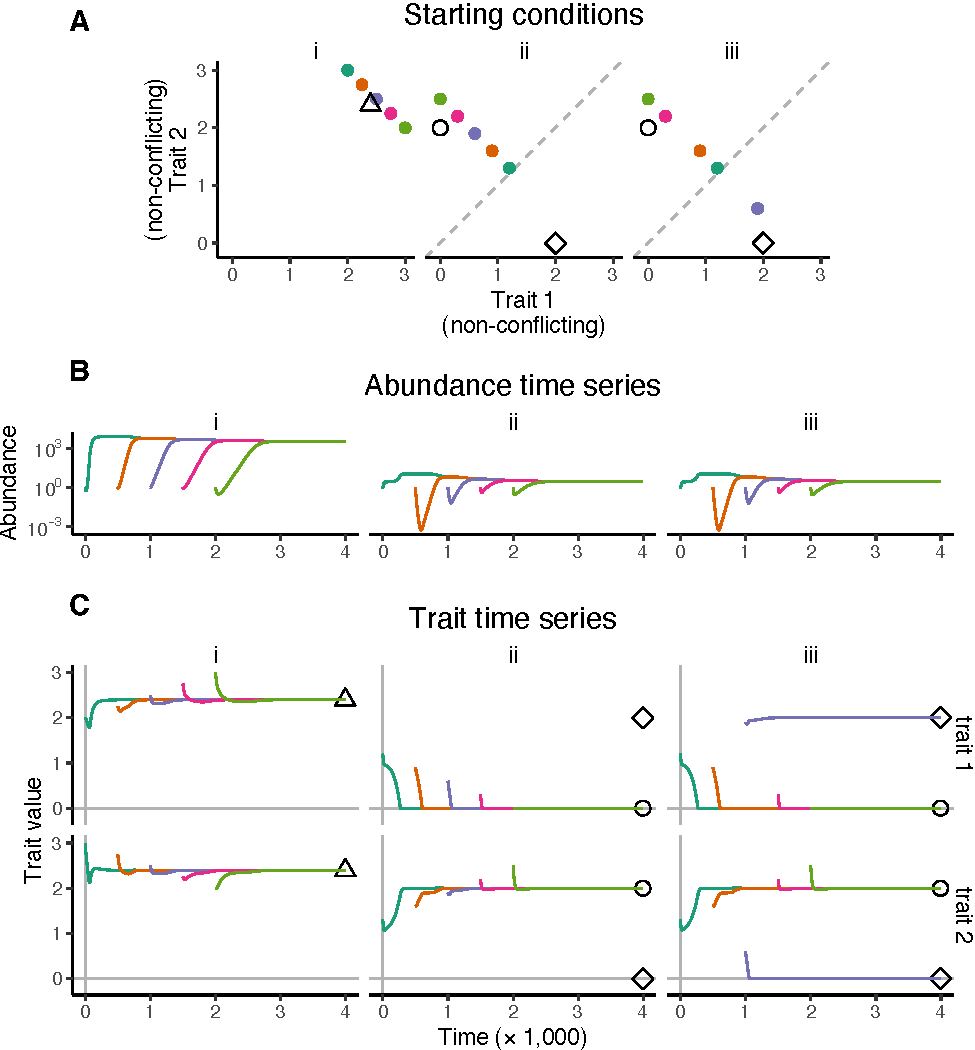
\includegraphics[width=\textwidth]{S1-cond_coexist_non-conflicting.pdf}
% \caption{Number of surviving species for 24 simulations of 2-trait 
%     communities
%     (A) after 50,000 generations for all permutations of the traits
%     being conflicting (``$-$'') or non-conflicting (``$+$''),
%     (B) after 50,000 generations for varying values of $d_2$ when 
%     $d_1$ is kept positive (i.e., trait 1 is kept non-conflicting), and
%     (C) through time with $d_2 = -10^{-2}$ and $d_2 = -10^{-4}$.
%     For all panels, $d_1 = 0.05$, $\eta = 0.6$, and species start with
%     random trait values ($\sim \text{N}(0,2)$ truncated $> 0$).
%     In (A), $d_2 = 0.1$.}
\caption{}
\label{fig:cond-coexist-non-conflicting}
\end{figure}


% \begin{figure}[ht!]
% \centering
% 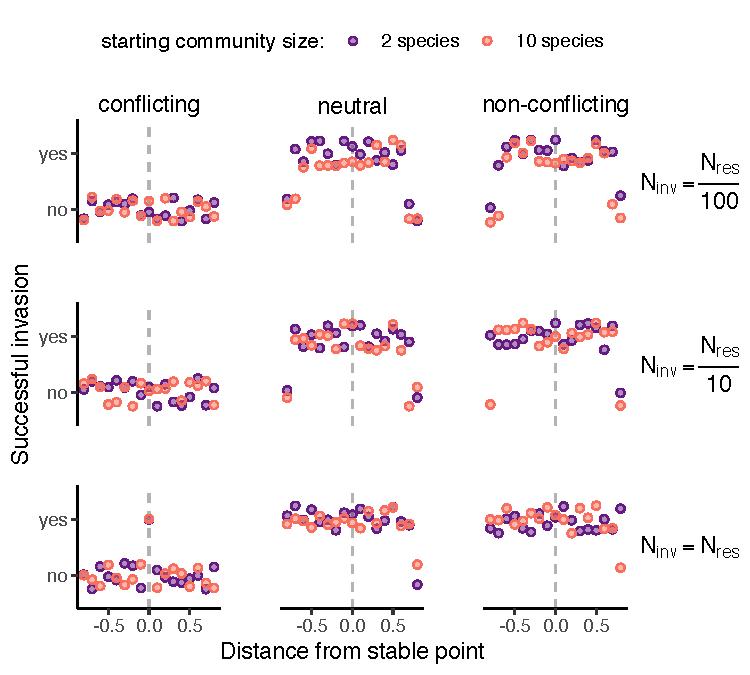
\includegraphics{S2-invasion.pdf}
% \caption{Invasion success for a 2-trait equilibrium community based on
%     the invader's starting distance from the equilibrium point in trait space.
%     Sub-panel columns indicate the type of evolution.
%     Sub-panels rows indicate the invaders' starting
%     abundances ($N_{eq}$) in relation to the residents'
%     abundances ($N_{res}$); all residents had the same
%     abundance.
%     Point color indicates the size of the resident community.
%     In these simulations, the resident community all had
%     trait values based on the analytical solutions for equilibria
%     in Appendix B.
%     The single invading species always had its first trait start
%     at the equilibrium value, but its second trait 
%     varied from
%     $-0.8$ to $0.8$ from the equilibrium value.
%     Simulations ran for 50,000 generations and assessed invasion 
%     success as the presence of the invader.
%     Here, $\eta = -0.6$, $d \in \{ -0.01, \; 0, \; 0.01 \}$.
% }
% \label{fig:invasion}
% \end{figure}

\begin{figure}[ht!]
\centering
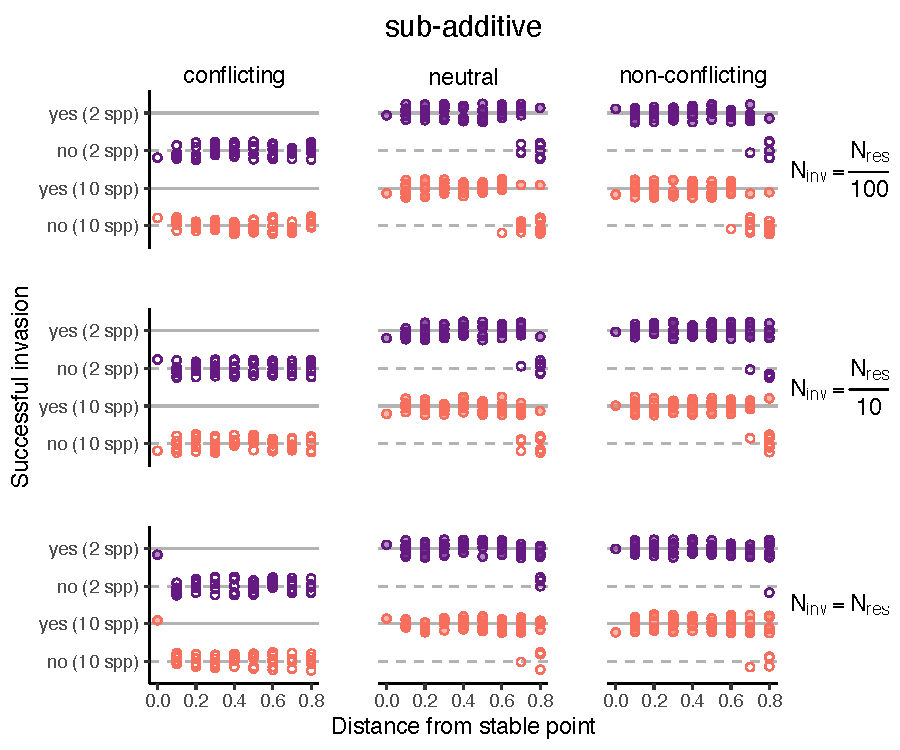
\includegraphics{S2-invasion_sub.pdf}
\caption{}
\label{fig:invasion-sub}
\end{figure}


\begin{figure}[ht!]
\centering
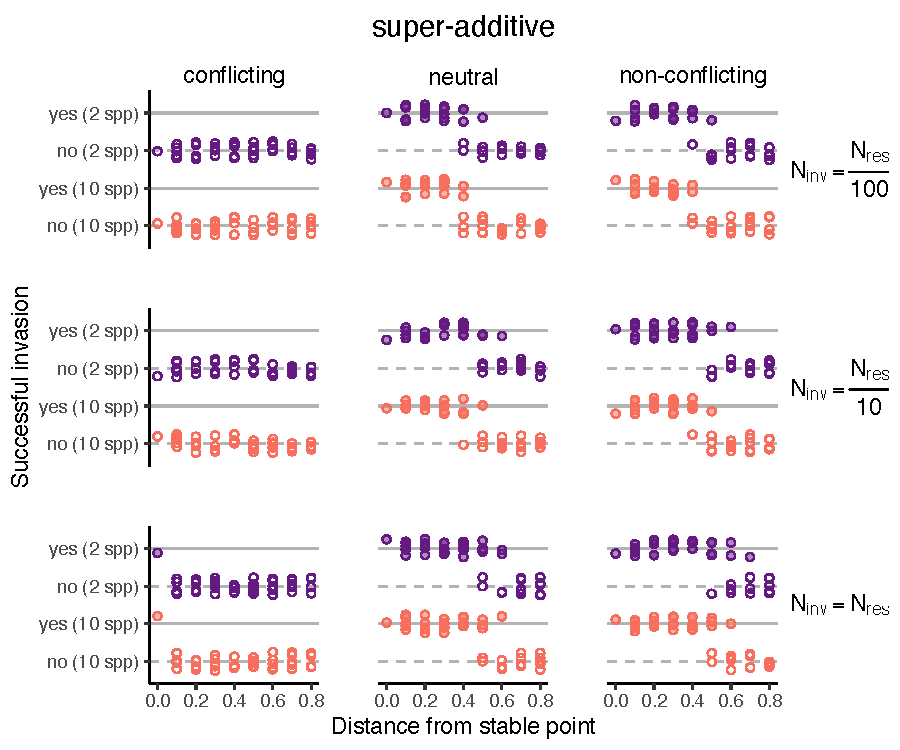
\includegraphics{S3-invasion_super.pdf}
\caption{}
\label{fig:invasion-super}
\end{figure}


% \clearpage
% \section*{Appendix D: Four-trait equilibrium solutions}

\renewcommand{\thefigure}{D\arabic{figure}}
\renewcommand{\theequation}{D\arabic{equation}}
\renewcommand{\thetable}{D\arabic{table}}
\setcounter{equation}{0}
\setcounter{figure}{0}
\setcounter{table}{0}



I haven't done these.




% ---------------------------------------------------------------------------------------
% ---------------------------------------------------------------------------------------
% Literature Cited
% ---------------------------------------------------------------------------------------
% ---------------------------------------------------------------------------------------

% You can either type your references following the examples below, or
% compile your BiBTeX database and paste the contents of your .bbl file
% here. The amnatnat.bst style file should work for this---but please
% let us know if you run into any hitches with it!
%
% If you upload a .bib file with your submission, please upload the .bbl
% file as well; this will be required for typesetting.
%
% The list below includes sample journal articles, book chapters, and
% Dryad references.

% \bibliographystyle{amnatnat.bst}
\bibliographystyle{ecology_letters.bst}
\clearpage
\bibliography{references.bib}




\clearpage


\renewcommand{\thefigure}{\arabic{figure}}
\renewcommand{\theequation}{\arabic{equation}}
\renewcommand{\thetable}{\arabic{table}}
\setcounter{equation}{0}
\setcounter{figure}{0}
\setcounter{table}{0}


\begin{figure}[ht!]
\centering
\includegraphics[width=0.9\textwidth,keepaspectratio]{1-diag.pdf}
\caption{Graphical model description.
% 
(a) Competition axes consist of suites of traits that together affect competition
similarly. Traits for a given axis can differ among species.
% 
(b) If species $i$ evolves an increase in a competition axis, this reduces its
per-capita growth rate and the effects of competition species $i$ experiences 
from other species in the community.
% 
(c) The cost associated with investing in multiple axes depends on whether 
tradeoffs are sub-additive, additive, or super-additive. 
Note that arrows within plots in this panel are all the same length.
% 
(d) Investment by species $i$ can either increase or decrease its effect on other
species in the community, depending on the type of competition axis it invests in.
Investment in an ameliorative axis by species $i$ reduces the effect of $i$ on all
other species.
The first example shown is behavioral avoidance of areas where heterospecifics
forage.
Next, investment in defensive traits that cause natural enemies to have 
differing effects on hosts can reduce apparent competition between hosts.
Lastly, multivariate traits can contribute to reduced resource-use overlap
between consumer species.
Investment in a conflicting axis by species $i$ increases the effect of $i$ on all
other species.
Traits that could contribute to conflicting axes include 
aggressive behavior toward heterospecifics near food sources,
chemical suppression of competitors for space, and
rapid growth that shades nearby plants.}
\label{fig:model-description}
\end{figure}




\begin{figure}[ht!]
\centering
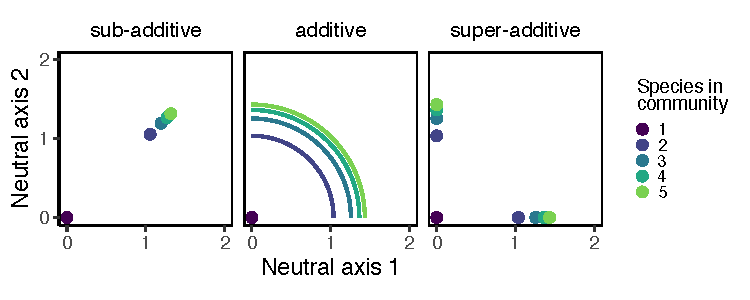
\includegraphics{2-outcomes_q2.pdf}
\caption{Unique axis values for surviving species in 2-axis communities
with varying numbers of species (indicated by color), and 
    for tradeoffs being sub-additive ($\eta < 0$), additive ($\eta = 0$), or 
    super-additive ($\eta > 0$).
    The lines in the additive case show the locations of the neutrally stable rings.
    Both axes are neutral (i.e., $\mathbf{d} = \{ 0, 0 \}$) to show only
    the effects of axis investment on the focal species.}
\label{fig:two-axis-outcomes}
\end{figure}






\begin{figure}[ht!]
\centering
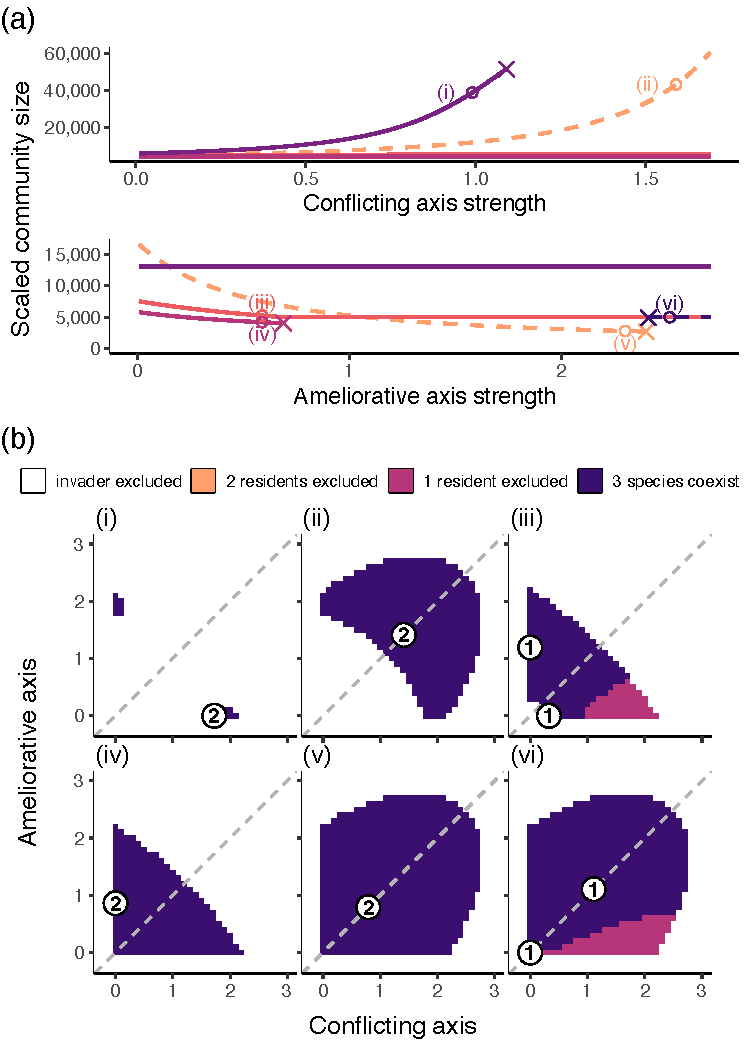
\includegraphics[width=0.6\textwidth,keepaspectratio]{3-comm.pdf}
\caption{Effects of axis strength and species investments on 
how permissive communities are to coexistence.
(a) How conflicting and ameliorative axis strength affect scaled community size,
for different communities (indicated by color) and tradeoffs
(solid for super-additive, dashed for sub-additive).
Scaled community size
($\sum_j^n{N_j \text{exp} \{ -\mathbf{v}_{j}^{\text{T}} \mathbf{D} \mathbf{v}_j \}}$)
represents the community abundance accounting
for the effect of species' axes on competition experienced by others in the
community. 
A lower value indicates greater invasibility.
In each sub-panel, the non-focal axis strength is fixed at 0.6.
Crosses indicate points where a community type is no longer stable,
and roman numerals indicate the community represented in panel (b).
(b) Invasibility of some communities representing how tradeoffs and species
investments influence coexistence.
Points in these plots indicate the axis values for equilibrium resident species, and 
numbers inside these points indicate the number of species at each point.
The background color shows what happens when a third species is added:
This invader either is excluded (white), 
excludes one or more residents (orange or pink), or 
coexists with residents to form a new, 3-species community (purple).
Note that ii and v show the same community at different axis strengths.
}
\label{fig:comms-d}
\end{figure}

\begin{figure}[ht!]
\centering
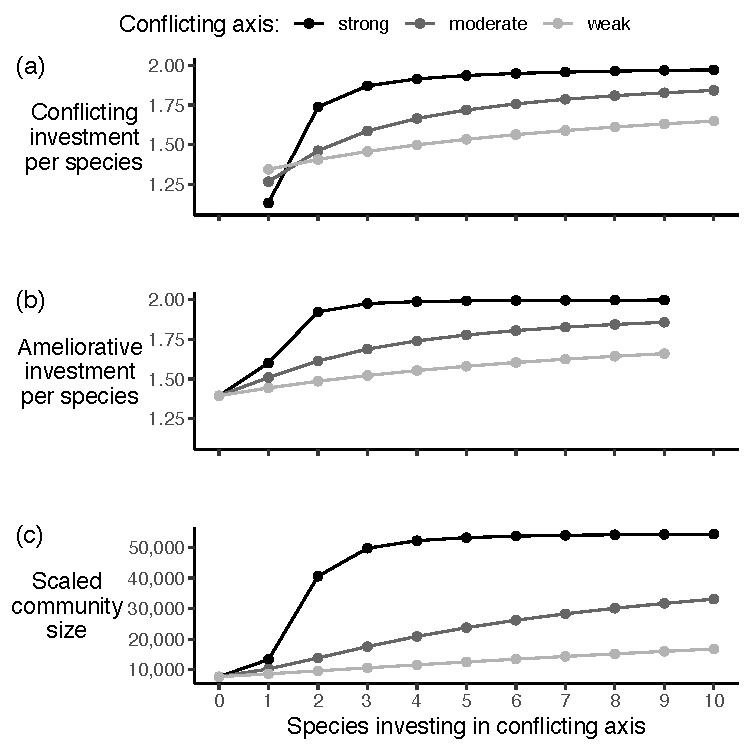
\includegraphics{4-stab.pdf}
\caption{Effects of the number of species investing in the conflicting axis
in 10-species communities with super-additive tradeoffs on 
(a) conflicting-axis investment per species,
(b) ameliorative-axis investment per species, and 
(c) scaled community size (inversely related to invasibility).
Color indicates whether the conflicting axis is strong ($d_{\text{conf}} = 1$),
moderate ($d_{\text{conf}} = 0.5$), or weak ($d_{\text{conf}} = 0.1$).
The ameliorative axis was fixed at $d_{\text{amel}} = 0.5$.
\label{fig:stabilizers}
}
\end{figure}




\begin{figure}[ht!]
\centering
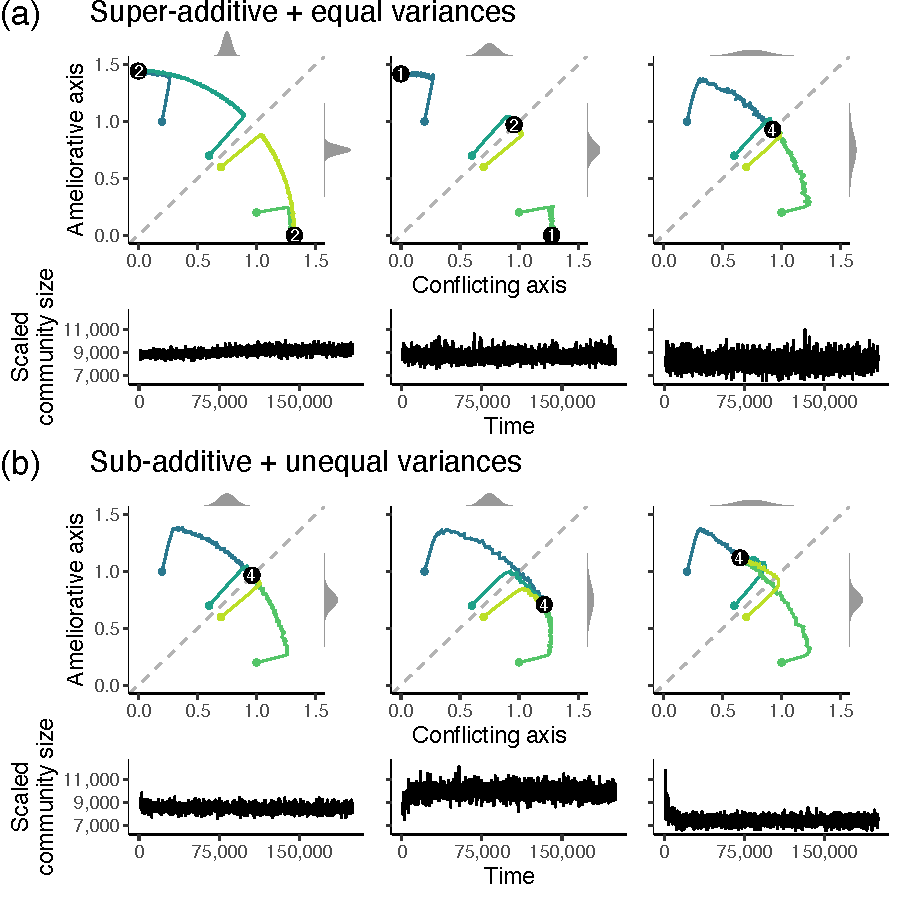
\includegraphics[width=0.9\textwidth,keepaspectratio]{5-stoch.pdf}
\caption{Examples of how stochasticity affects tradeoffs, 
possible communities, and invasibility.
Shown are the effects of axis-evolution stochasticity when
(a) variance is equal among axes and tradeoffs are super-additive and 
(b) variance is unequal among axes and tradeoffs are sub-additive.
The upper row of each sub-panel shows the trajectories in axis space
for 4 species started under each scenario.
Open points indicate starting axis values.
Closed points indicate ending axis values, and 
numbers inside these points indicate the number of species at each point.
Gray shaded curves outside each plot show the probability density for
the normal distributions used to generate stochasticity in the
conflicting (top curve) or ameliorative (right curve) axis.
The lower row shows scaled community size through time for each community
in the top row;
a lower scaled community size indicates greater invasibility.
The first 1,000 time steps are removed to better highlight differences
between communities after the initial period of population expansions.
}
\label{fig:stochasticity}
\end{figure}



\clearpage


\section*{Supplemental Information}

\renewcommand{\thefigure}{S\arabic{figure}}
\renewcommand{\theequation}{S\arabic{equation}}
\renewcommand{\thetable}{S\arabic{table}}
\setcounter{equation}{0}
\setcounter{figure}{0}
\setcounter{table}{0}


% Note: this should go into a separate document eventually

\section*{Matrix derivatives in quantitative genetics equations}

As in the main text, $^{\textrm{T}}$ indicates transposition,
multiplication between matrices is always matrix multiplication, and
bold face indicates a matrix.
Also note that both $\mathbf{C}$ and $\mathbf{D}$ are symmetrical,
so $\mathbf{C} + \mathbf{C}^{\textrm{T}} = 2 \; \mathbf{C}$ and
$\mathbf{D} + \mathbf{D}^{\textrm{T}} = 2 \; \mathbf{D}$.


We can combine the equations in the Methods section as such:

\begin{equation} \label{eq:fitness-full}
\begin{split}
    F_{i,t+1} &= \exp \left\{
        r_0 - f \; \mathbf{v}_{i,t}^{\textrm{T}} \; \mathbf{C} \; \mathbf{v}_{i,t} -
        \alpha_0 \;\textrm{e}^{- \mathbf{v}_{i,t}^{\textrm{T}} \mathbf{v}_{i,t} } \mathbf{\Omega}_{i,t}
        \right\} \\
        \mathbf{\Omega}_{i,t} &\equiv N_{i,t} +
            \sum_{j \ne i}^{n}{ N_{j,t} \textrm{e}^{
            - \mathbf{v}_{j,t}^{\textrm{T}}
            \mathbf{D} \mathbf{v}_{j,t} } }
        \textrm{.}
\end{split}
\end{equation}

\noindent where $\mathbf{\Omega}_i$ represents the community abundance scaled
for the effect other species' axes values has on competition
experienced by species $i$.
Hereafter we will refer to $\mathbf{\Omega}_i$ as the scaled community size.




\subsection*{Axis evolution}

From the main text and above, we know that

\begin{equation}\label{eq:main-text-info-axis-change}
\begin{split}
    F_{i,t+1} &= \exp \left\{
        r_0 - f \; \mathbf{v}_{i,t}^{\textrm{T}} \; \mathbf{C} \; \mathbf{v}_{i,t} -
        \alpha_0 \;\textrm{e}^{- \mathbf{v}_{i,t}^{\textrm{T}} \mathbf{v}_{i,t} } \mathbf{\Omega}_{i,t}
        \right\} \\
    \mathbf{v}_{i,t+1} &= \mathbf{v}_{i,t} + \left( \frac{1}{F_{i,t+1}}
        \frac{\partial F_{i,t+1}}{\partial \mathbf{v}_{i,t}} \right) \sigma^2_i
    \textrm{.}
\end{split}
\end{equation}


The partial derivative of fitness in relation to axes for species $i$ is


\begin{equation*}
\begin{split}
    \frac{\partial F_{i,t+1}}{\partial \mathbf{v}_{i,t}} &=
        \exp \left\{
            r_0
            - f \mathbf{v}_{i,t}^{\textrm{T}} \mathbf{C} \mathbf{v}_{i,t}
            - \alpha_0  \mathbf{\Omega}_{i,t} \,
                \textrm{e}^{- \mathbf{v}_{i,t}^{\textrm{T}} \mathbf{v}_{i,t}}
        \right\}
        \frac{\partial \!
            \left(
                r_0
                - f \; \mathbf{v}_{i,t}^{\textrm{T}} \; \mathbf{C} \; \mathbf{v}_{i,t}
                - \alpha_0 \; \mathbf{\Omega}_{i,t} \;
                    \textrm{e}^{- \mathbf{v}_{i,t}^{\textrm{T}} \mathbf{v}_{i,t}}
            \right)
            }{ \partial \mathbf{v}_{i,t} } \\
     &=
        \exp \left\{
            r_0
            - f \mathbf{v}_{i,t}^{\textrm{T}} \mathbf{C} \mathbf{v}_{i,t}
            - \alpha_0  \mathbf{\Omega}_{i,t} \,
                \textrm{e}^{- \mathbf{v}_{i,t}^{\textrm{T}} \mathbf{v}_{i,t}}
        \right\}
        \left[
            - 2 f \mathbf{v}_{i,t}^{\textrm{T}} \mathbf{C}
            - \alpha_0 \, \mathbf{\Omega}_{i,t} \,
                \textrm{e}^{- \mathbf{v}_{i,t}^{\textrm{T}} \mathbf{v}_{i,t} } \:
                \frac{\partial \! \left( - \mathbf{v}_{i,t}^{\textrm{T}} \mathbf{v}_{i,t} \right)
                    }{ \partial \mathbf{v}_{i,t} }
        \right] \\[2ex]
    \frac{ \partial F_{i,t} }{ \partial \mathbf{v}_{i,t} } &=
        \exp \left\{
            r_0
            - f \mathbf{v}_{i,t}^{\textrm{T}} \mathbf{C} \mathbf{v}_{i,t}
            - \alpha_0  \mathbf{\Omega}_{i,t} \,
                \textrm{e}^{- \mathbf{v}_{i,t}^{\textrm{T}} \mathbf{v}_{i,t}}
        \right\}
        \left[
            2 \alpha_0 \mathbf{\Omega}_{i,t} \,
                \textrm{e}^{- \mathbf{v}_{i,t}^{\textrm{T}} \mathbf{v}_{i,t}} \:
                \mathbf{v}_{i,t}^{\textrm{T}}
            - 2 f \mathbf{v}_{i,t}^{\textrm{T}} \mathbf{C}
        \right]
    \textrm{.}
\end{split}
\end{equation*}



Combining above with equation \ref{eq:main-text-info-axis-change}, we find that axis values at
time $t+1$ are

\begin{equation} \label{eq:supp-axis-change-full}
    \mathbf{v}_{i,t+1} = \mathbf{v}_{i,t} + 2 \sigma_i^2
    \left(
        \alpha_0 \, \mathbf{\Omega}_{i,t} \:
            \textrm{e}^{- \mathbf{v}_{i,t}^{\textrm{T}} \mathbf{v}_{i,t}} \:
            \mathbf{v}_{i,t}^{\textrm{T}}
        - f \, \mathbf{v}_{i,t}^{\textrm{T}} \: \mathbf{C}
    \right)
    \textrm{.}
\end{equation}


\subsection*{Jacobian matrix}

The $n(q+1) \times n(q+1)$ Jacobian matrix consists of 

\begin{itemize}
\item $n^2$ blocks of size $q \times q$ containing
    $\partial \mathbf{v}_{i,t+1} / \partial \mathbf{v}_{\zeta,t}$
\item $n^2$ blocks of size $1 \times q$ containing
    $\partial \mathbf{v}_{i,t+1} / \partial N_{\zeta,t}$
\item $n^2$ blocks of size $q \times 1$ containing
    $\partial N_{i,t+1} / \partial \mathbf{v}_{\zeta,t}$
\item $n^2$ blocks of size $1 \times 1$ containing
    $\partial N_{i,t+1} / \partial N_{\zeta,t}$
\end{itemize}


for all $i \in \{ 1, \: \ldots \, , \: n \}$
and $\zeta \in \{ 1, \: \ldots \, , \: n \}$.


The partial derivatives of species $i$ axes at time $t+1$ with respect
to species $i$ axes at time $t$ are

\begin{equation*}
\begin{split}
    \frac{ \partial \, \mathbf{v}_{i,t+1} }{ \partial \, \mathbf{v}_{i,t} } &=
        \frac{ \partial \, \mathbf{v}_{i,t} }{ \partial \, \mathbf{v}_{i,t} } +
        2 \; \sigma_i^2
        \left(
            \frac{ \partial \;
                \alpha_0 \; \mathbf{\Omega}_{i,t} \;
                    \textrm{e}^{-\mathbf{v}_{i,t}^{\textrm{T}} \mathbf{v}_{i,t}} \,
                    \mathbf{v}_{i,t}^{\textrm{T}}}{\partial \; \mathbf{v}_{i,t} } -
            \frac{ \partial \; f \, \mathbf{v}_{i,t}^{\textrm{T}} \mathbf{C}}{\partial \; \mathbf{v}_{i,t} }
        \right) \\
    &=
        \mathbf{I} +
        2 \; \sigma_i^2
        \left[
            \alpha_0 \; \mathbf{\Omega}_{i,t} \,
            \left(
                \textrm{e}^{-\mathbf{v}_{i,t}^{\textrm{T}} \mathbf{v}_{i,t}} +
                \frac{ \partial \;
                        \textrm{e}^{-\mathbf{v}_{i,t}^{\textrm{T}} \mathbf{v}_{i,t}}
                        }{\partial \; \mathbf{v}_{i,t} } \, \mathbf{v}_{i,t}^{\textrm{T}}
            \right) -
            f \, \mathbf{C}^{\textrm{T}}
            \right] \\[2ex]
    \frac{ \partial \, \mathbf{v}_{i,t+1} }{ \partial \, \mathbf{v}_{i,t} } &= \mathbf{I} + 2 ~ \sigma_i^2 ~
        \left[
            \alpha_0 ~ \mathbf{\Omega}_{i,t} ~ \textrm{e}^{ - \mathbf{v}_{i,t}^{\textrm{T}} \mathbf{v}_{i,t} }
            \left(
                \mathbf{I} - 2 ~ \mathbf{v}_{i,t} \mathbf{v}_{i,t}^{\textrm{T}}
            \right) -
            f \: \mathbf{C}^{\textrm{T}}
        \right]
    \textrm{,}
\end{split}
\end{equation*}

\noindent where $\mathbf{I}$ is a $q \times q$ identity matrix.


Next we have the partial derivatives of species $i$ axes at time $t+1$ with respect to 
species $k$ axes at time $t$, where $k \ne i$.
To calculate this, it's useful to rearrange equation \ref{eq:axes-change-full} and
extract the portion that includes $\mathbf{v}_{k,t}$:


\begin{equation*}
\begin{split}
    \mathbf{v}_{i,t+1} &= \mathbf{v}_{i,t} + 2 \; \sigma_i^2
    \left[
        \left(
            N_{k,t} \; \textrm{e}^{ -\mathbf{v}_{k,t}^{\textrm{T}} \mathbf{D}
            \mathbf{v}_{k,t} } + \mathbf{\Phi}_{i,t}
        \right)
        \left(
            \alpha_0 \; \textrm{e}^{-\mathbf{v}_{i,t}^{\textrm{T}}
            \mathbf{v}_{i,t} } \; \mathbf{v}_{i,t}^{\textrm{T}}
        \right)
        - f \: \mathbf{v}_{i,t}^{\textrm{T}} \mathbf{C}
    \right] \\
    \mathbf{\Phi}_{i,t} &= N_{i,t} + \sum_{j \ne i, j \ne k}^{n}{
        N_{j,t} \; \textrm{e}^{- \mathbf{v}_{j,t}^{\textrm{T}}
        \mathbf{D} \mathbf{v}_{j,t} } }
    \textrm{.}
\end{split}
\end{equation*}

From this we calculated the partial derivative of $\mathbf{v}_{i,t+1}$ in relation to
$\mathbf{v}_{k,t}$


\begin{equation*}
\begin{split}
    \frac{ \partial \: \mathbf{v}_{i,t+1} }{ \partial \: \mathbf{v}_{k,t} } &=
        \frac{ \partial \: \mathbf{v}_{i,t} }{ \partial \: \mathbf{v}_{k,t} } +
        2 \; \sigma_i^2 \;
        \left[
            \frac{ \partial \:
                \left(
                    N_{k,t} \textrm{e}^{- \mathbf{v}_{k,t}^{\textrm{T}} \mathbf{D}
                    \mathbf{v}_{k,t}} + \mathbf{\Phi}_{i,t}
                \right)
                \left(
                    \alpha_0 \; \textrm{e}^{ - \mathbf{v}_{i,t}^{\textrm{T}}
                    \mathbf{v}_{i,t} } \mathbf{v}_{i,t}^{\textrm{T}}
                \right)
            }{ \partial \:  \mathbf{v}_{k,t} } -
            \frac{ \partial \:  f \, \mathbf{v}_{i,t}^{\textrm{T}} \mathbf{C} }{
            \partial \: \mathbf{v}_{k,t} }
        \right] \\
    &= 2 \; \sigma_i^2 \; \alpha_0 \; N_{k,t} \; \mathbf{v}_{i,t} \;
        \textrm{e}^{ - \mathbf{v}_{i,t}^{\textrm{T}}
        \mathbf{v}_{i,t} } \; 
        \frac{ \partial \:
                \textrm{e}^{
                    - \mathbf{v}_{k,t}^{\textrm{T}} \mathbf{D} \mathbf{v}_{k,t}
                    }
            }{ \partial \:  \mathbf{v}_{k,t} } \\
    &= 2 \; \sigma_i^2 \; \alpha_0 \; N_{k,t} \; \mathbf{v}_{i,t} \;
        \textrm{e}^{
                    - \mathbf{v}_{k,t}^{\textrm{T}} \mathbf{D} \mathbf{v}_{k,t}
                    - \mathbf{v}_{i,t}^{\textrm{T}} \mathbf{v}_{i,t}
                } \;
        \left[ 
            - 2 \, \mathbf{v}_{k,t}^{\textrm{T}} \, \mathbf{D}
        \right] \\
    \frac{ \partial \: \mathbf{v}_{i,t+1} }{ \partial \: \mathbf{v}_{k,t}} &=
        -4 \; \sigma_i^2 \; \alpha_0 \; N_{k,t} \; \mathbf{v}_{i,t} \;
        \textrm{e}^{
                    - \mathbf{v}_{k,t}^{\textrm{T}} \mathbf{D} \mathbf{v}_{k,t}
                    - \mathbf{v}_{i,t}^{\textrm{T}} \mathbf{v}_{i,t}
                } \;
        \mathbf{v}_{k,t}^{\textrm{T}} \; \mathbf{D}
    \textrm{.} \\
\end{split}
\end{equation*}

The partial derivatives of species $i$ axes in relation to species $i$ 
and species $k$ abundances are

\begin{equation*}
\begin{split}
    \frac{ \partial \: \mathbf{v}_{i,t+1} }{ \partial \: N_{i,t} } &=
        2 \; \sigma_i^2 \; \alpha_0 \; \mathbf{v}_{i,t} \;
        \textrm{e}^{ - \mathbf{v}_{i,t}^{\textrm{T}} \mathbf{v}_{i,t} } \\
    \frac{ \partial \: \mathbf{v}_{i,t+1} }{ \partial \: N_{k,t} } &=
        2 \; \sigma_i^2 \; \alpha_0 \; \mathbf{v}_{i,t} \;
        \textrm{e}^{ - \mathbf{v}_{k,t}^{\textrm{T}} \mathbf{D} \mathbf{v}_{k,t}
            - \mathbf{v}_{i,t}^{\textrm{T}} \mathbf{v}_{i,t} }
    \textrm{.} \\
\end{split}
\end{equation*}




For partial derivatives of abundances in relation to the other state variables,
we use the following equations from above:


\begin{equation*}
\begin{split}
    N_{i,t+1} &= N_{i,t} \; F_{i,t+1} \\
    F_{i,t+1} &=  \exp \left\{
        r_0 - f \, \mathbf{v}_{i,t}^{\text{T}} \, \mathbf{C} \, \mathbf{v}_{i,t} - 
        \alpha_0 \, \text{e}^{-\mathbf{v}_{i,t}^{\text{T}} \, \mathbf{v}_{i,t}} \,
        \Omega_{i,t}
    \right\} \\
    \Omega_{i,t} &= N_{i,t} + \sum_{j \ne i}^{n}{ N_j \:
        \text{e}^{- \mathbf{v}_{j,t}^{\text{T}} \, \mathbf{D} \, \mathbf{v}_{j,t} } }
    \textrm{.} \\
\end{split}
\end{equation*}



Using these, we have the following derivatives of abundances in relation
to axes:

\begin{equation*}
\begin{split}
    \frac{ \partial N_{i,t+1} }{ \partial \mathbf{v}_{i,t} } &= 
        2 \, F_{i,t+1} \,  N_{i,t}
        \left(
            \alpha_0 \, \Omega_{i,t} \, \text{e}^{ -\mathbf{v}_{i,t}^{\text{T}}
            \mathbf{v}_{i,t} } \, \mathbf{v}_{i,t}^{\text{T}}
            - f \, \mathbf{v}_{i,t}^{\text{T}} \, \mathbf{C}
        \right) \\
    \frac{ \partial N_{i,t+1} }{ \partial \mathbf{v}_{k,t} } &= 
        2 \, F_{i,t+1} \, N_{i,t} \, N_{k,t} \, \alpha_0 \: 
        \text{e}^{ -\mathbf{v}_{i,t}^{\text{T}} \mathbf{v}_{i,t} -
            \mathbf{v}_{k,t}^{\text{T}} \mathbf{D} \mathbf{v}_{k,t} } \:
        \mathbf{v}_{k,t}^{\text{T}} \, \mathbf{D}
    \textrm{.}
\end{split}
\end{equation*}

We also have the following derivatives of abundances at time $t+1$ in relation
to those at time $t$:

\begin{equation*}
\begin{split}
    \frac{ \partial N_{i,t+1} }{ \partial N_{i,t} } &= 
        F_{i,t+1}
        \left(
            1 - N_{i,t} \: \alpha_0 \: 
            \text{e}^{ -\mathbf{v}_{i,t}^{\text{T}} \mathbf{v}_{i,t} } 
        \right) \\
    %
    \frac{ \partial N_{i,t+1} }{ \partial N_{k,t} } &= 
        - F_{i,t+1} \: N_{i,t} \: \alpha_0 \: 
        \text{e}^{ -\mathbf{v}_{i,t}^{\text{T}} \mathbf{v}_{i,t} -
            \mathbf{v}_{k,t}^{\text{T}} \mathbf{D} \mathbf{v}_{k,t} } 
    \textrm{.}
\end{split}
\end{equation*}











% ========================================================================================
% ========================================================================================
% ========================================================================================
% ========================================================================================
% ========================================================================================
% ========================================================================================
% ========================================================================================






\section*{Two-axis equilibrium solutions}

For these solutions, we will no longer use matrix notation.
Also, since all axes have the same costs, benefits, and
non-additive effects, solutions for axis 1 and 2 are the same.
Only solutions for axis 1 are presented.
We use a hat to distinguish equilibrium values
($\hat{Z}$ for parameter $Z$).
Lastly, because $\mathbf{C}$ is symmetrical, only has 2 rows and columns, and
differs only on the off-diagonals, there is only one $\eta$ value.


\subsection*{Axis values}

The two axes for species $i$ change as follows:

\begin{equation*}
\begin{split}
    v_{i1,t+1} &= v_{i1,t} + 2 \; \sigma^2
    \left[
        \alpha_0 \; \Omega_{i,t} \;
            \textrm{e}^{-v_{i1,t}^2 - v_{i2,t}^2} \; v_{i1,t}
        - f \; ( v_{i1,t} + \eta \; v_{i2,t} )
    \right] \\
    v_{i2,t+1} &= v_{i2,t} + 2 \; \sigma^2
    \left[
        \alpha_0 \; \Omega_{i,t} \;
            \textrm{e}^{-v_{i2,t}^2 - v_{i1,t}^2} \; v_{i2,t}
        - f \; ( v_{i2,t} + \eta \; v_{i1,t} )
    \right] \\
    \Omega_{i,t} &\equiv N_{i,t} +
        \sum_{j \ne i}^{n}{ N_{j,t} \; \textrm{e}^{
                - d_1 v_{j1,t}^2 - d_2 v_{j2,t}^2 } }
    \textrm{.}
\end{split}
\end{equation*}


We'll now drop indices for species and time because we are
focusing on just one species and time point.



At equilibrium (assuming that $\sigma > 0$),

\begin{equation}
\begin{split}
    0 &= \alpha_0 \; \hat{\Omega} \;
            \textrm{e}^{-\hat{v}_{1}^2 - \hat{v}_{2}^2} \; \hat{v}_{1}
        - f \; ( \hat{v}_{1} + \eta \; \hat{v}_{2} ) \\
    0 &=
        \alpha_0 \; \hat{\Omega} \;
            \textrm{e}^{-\hat{v}_{2}^2 - \hat{v}_{1}^2} \; \hat{v}_{2}
        - f \; ( \hat{v}_{2} + \eta \; \hat{v}_{1} )
    \textrm{.}
\end{split}
\label{eq:two-axes-v-eq1}
\end{equation}


\noindent Thus, we have

\begin{equation*}
\begin{split}
    \alpha_0 \; \hat{\Omega} \; \textrm{e}^{-\hat{v}_{1}^2 - \hat{v}_{2}^2} &=
        \frac{ f \; ( \hat{v}_{1} + \eta \; \hat{v}_{2} ) }{ \hat{v}_{1} } \\
    \alpha_0 \; \hat{\Omega} \; \textrm{e}^{-\hat{v}_{1}^2 - \hat{v}_{2}^2} &=
        \frac{ f \; ( \hat{v}_{2} + \eta \; \hat{v}_{1} ) }{ \hat{v}_{2} }
    \textrm{.}
\end{split}
\end{equation*}


\noindent Combining these leads to

\begin{equation*}
\begin{split}
    f \; ( \hat{v}_{1} + \eta \; \hat{v}_{2} ) \; \hat{v}_{2} &=
        f \; ( \hat{v}_{2} + \eta \; \hat{v}_{1} ) \; \hat{v}_{1} \\
    f \hat{v}_{1} \hat{v}_{2} + \eta \hat{v}_{2}^2 &=
        f \hat{v}_{1} \hat{v}_{2} + \eta \hat{v}_{1}^2 \\
    \eta \hat{v}_{2}^2 &= \eta \hat{v}_{1}^2 \\
    \hat{v}_{1} &= \hat{v}_{2}
    \textrm{.}
\end{split}
\end{equation*}

Since all $v$ must be $\ge 0$ (hence no $\pm$ in the equation above),
either $\hat{v}_{1} = \hat{v}_{2}$ or not (when $\eta = 0$).
Plugging in $\hat{v}_{1} = \hat{v}_{2}$ into equation \ref{eq:two-axes-v-eq1}
gives us

\begin{equation*}
\begin{split}
    0 &= \alpha_0 \; \hat{\Omega} \; \textrm{e}^{-2 \; \hat{v}_{1}^2 } \; \hat{v}_{1}
        - f \; ( \hat{v}_{1} + \eta \; \hat{v}_{1} ) \\
    &= \hat{v}_{1} \left[ \alpha_0 \; \hat{\Omega} \; \textrm{e}^{-2 \; \hat{v}_{1}^2 }
        - f \; ( 1 + \eta ) \right]
    \textrm{.}
\end{split}
\end{equation*}

\noindent One solution is $\hat{v}_{1} = 0$, but if $\hat{v}_{1} \ne 0$


\begin{equation}
\begin{split}
    \alpha_0 \; \hat{\Omega} \; \textrm{e}^{-2 \; \hat{v}_{1}^2 } &=
        f \; ( 1 + \eta ) \\
    -2 \; \hat{v}_{1}^2 &=
        \log \left( \frac{ f \; ( 1 + \eta ) }{ \alpha_0 \; \hat{\Omega} } \right) \\
    \hat{v}_{1} &= \sqrt{\frac{1}{2}
        \log \left( \frac{ \alpha_0 \; \hat{\Omega} }{ f \; ( 1 + \eta ) } \right) }
    \textrm{.}
\end{split}
\label{eq:two-axes-v-eq5}
\end{equation}



When $\eta = 0$ and at least one of the two axes $\ne 0$,
axes are constrained by their distance
from the origin: $\sqrt{\hat{v}_{1}^2 + \hat{v}_{2}^2}$.
When $\hat{v}_{1} \ne 0$, this distance is

\begin{equation*}
\begin{split}
    0 &= \alpha_0 \; \hat{\Omega} \;
            \textrm{e}^{-\hat{v}_{1}^2 - \hat{v}_{2}^2} \; \hat{v}_{1}
        - f \; \hat{v}_{1} \\
    0 &= \alpha_0 \; \hat{\Omega} \;
        \textrm{e}^{- ( \hat{v}_{1}^2 + \hat{v}_{2}^2) }
        - f \\
    \log \left( \frac{\alpha_0 \; \hat{\Omega}}{ f } \right) &=
        \hat{v}_{1}^2 + \hat{v}_{2}^2 \\
     \sqrt{ \hat{v}_{1}^2 + \hat{v}_{2}^2 } &=
        \sqrt{ \log \left( \frac{\alpha_0 \; \hat{\Omega}}{ f } \right)}
    \textrm{.}
\end{split}
\end{equation*}

\noindent So the relationship between axes when $\eta = 0$ is

$$
    \hat{v}_{1} =
    \sqrt{
        \log \left( \frac{\alpha_0 \; \hat{\Omega}}{ f } \right) -
        \hat{v}_{2}^2
    }
    \textrm{,}
$$

\noindent when $\hat{v}_{2}^2 \ge \log (\alpha_0 \hat{\Omega} / f)$.

We've shown solutions for when $v_1 = v_2$ and when $\eta = 0$, but
when one axis is zero but the other is not (and $\eta$ isn't necessarily 0),
we get the following (for $v_1 \ne 0$ and $v_2 = 0$):

\begin{equation}
\begin{split}
    0 &=
        \alpha_0 \; \hat{\Omega} \;
            \textrm{e}^{-\hat{v}_{1}^2 - \hat{v}_{2}^2} \; \hat{v}_{1}
        - f \; ( \hat{v}_{1} + \eta \; \hat{v}_{2} ) \\
    0 &=
        \alpha_0 \; \hat{\Omega} \;
            \textrm{e}^{-\hat{v}_{1}^2} \; \hat{v}_{1}
        - f \; \hat{v}_{1} \\
    0 &=
        \alpha_0 \; \hat{\Omega} \;
            \textrm{e}^{-\hat{v}_{1}^2} - f \\
    \frac{f}{\alpha_0 \; \hat{\Omega}} &=
         \frac{1}{\textrm{e}^{\hat{v}_{1}^2}} \\
    \hat{v}_{1} &= \sqrt{ \log \left( \frac{\alpha_0 \; \hat{\Omega}}{f} \right) }
\end{split}
\label{eq:two-axes-v1-nonzero-v2-zero}
\end{equation}







% -----------------------------------------------------------------
% -----------------------------------------------------------------







\subsection*{Scaled community size}

Fitness for the species is written as

$$
    F = \exp \left\{
        r_0 - f ( {v}_{1}^2 + 2 \eta {v}_{1} {v}_{2} + {v}_{2}^2 ) -
        \alpha_0 \, \textrm{e}^{ - {v}_{1}^2 - {v}_{2}^2 } \, \Omega
    \right\}
    \textrm{.}
$$


\noindent At equilibrium,

\begin{equation}
    0 = r_0 - f ( \hat{v}_{1}^2 + 2 \eta \hat{v}_{1} \hat{v}_{2} + \hat{v}_{2}^2 ) -
        \alpha_0 \, \textrm{e}^{ - {v}_{1}^2 - {v}_{2}^2 } \, \Omega
    \textrm{.}
\label{eq:two-axes-omega-equil-start}
\end{equation}


\noindent When $\hat{v}_1 = \hat{v}_2$, we can insert our answer from
\ref{eq:two-axes-v-eq5} to get

\begin{equation*}
\begin{split}
    0 &= r_0 - 2 \; f \; \hat{v}_{1}^2 ( 1 + \eta ) -
        \alpha_0 \textrm{e}^{ -2 \; \hat{v}_{1}^2 } \hat{\Omega} \\
    r_0 &= 2 f ( 1 + \eta ) \left[
        \frac{1}{2}
        \log \left( \frac{ \alpha_0 \; \hat{\Omega} }{ f \; ( 1 + \eta ) } \right)
    \right] +
        \alpha_0 \textrm{e}^{ -2 \;
            \left[
                \frac{1}{2} \log \left(
                    \frac{ \alpha_0 \; \hat{\Omega} }{ f \; ( 1 + \eta ) }
                \right)
            \right]
        } \hat{\Omega} \\
    r_0 &= f ( 1 + \eta ) \log \left(
        \frac{ \alpha_0 \; \hat{\Omega} }{ f \; ( 1 + \eta ) }
    \right) + f ( 1 + \eta ) \\
    \frac{  r_0 - f ( 1 + \eta ) }{ f ( 1 + \eta ) } &=
        \log \left(
        \frac{ \alpha_0 \; \hat{\Omega} }{ f \; ( 1 + \eta ) }
        \right) \\
    \hat{\Omega} &= \frac{ f \; ( 1 + \eta ) }{ \alpha_0 } \;
        \textrm{e}^{\frac{  r_0 }{ f ( 1 + \eta ) } - 1 }
    \textrm{.}
\end{split}
\end{equation*}

Thus, when $\hat{v}_1 = \hat{v}_2$,
$$
\hat{\Omega} = \frac{ f \; ( 1 + \eta ) }{ \alpha_0 } \;
        \textrm{e}^{\frac{ r_0 }{ f ( 1 + \eta ) } - 1 }
    \textrm{.}
$$


\noindent When $\eta = 0$,

$$
    \hat{\Omega} = \frac{ f }{ \alpha_0 } \; \textrm{e}^{\frac{ r_0 }{ f } - 1 }
    \textrm{.}
$$



If instead $v_1 = 0$ and $v_2 \ne 0$, we can start by simplifying equation
\ref{eq:two-axes-omega-equil-start}

\begin{equation*}
\begin{split}
    0 &= r_0 - f \hat{v}_{1}^2 -
        \alpha_0 \textrm{e}^{ - \hat{v}_{1}^2 } \hat{\Omega} \\
    \hat{\Omega} &= \frac{ r_0 - f \hat{v}_{1}^2 }{ \alpha_0 } \textrm{e}^{ \hat{v}_{1}^2 }
    \textrm{.}
\end{split}
\end{equation*}

Now we combine this with \ref{eq:two-axes-v1-nonzero-v2-zero}

\begin{equation*}
\begin{split}
    \hat{\Omega} &= \frac{ r_0 - f \log \left( \frac{\alpha_0 \hat{\Omega}}{f} \right) }{
        \alpha_0 } \left( \frac{\alpha_0 \; \hat{\Omega}}{f} \right) \\
    1 &= \frac{ r_0 }{ f } - \log \left( \frac{\alpha_0 \hat{\Omega}}{f} \right) \\
    \hat{\Omega} &= \frac{f}{\alpha_0} \textrm{e}^{\frac{r_0}{f} - 1}
    \textrm{.}
\end{split}
\end{equation*}











% -----------------------------------------------------------------
% -----------------------------------------------------------------








\subsection*{Combined solutions}

When $\hat{v}_1 = \hat{v}_2$,

\begin{equation}  \label{eq:two-axes-finals-eta-negative}
\begin{split}
    \hat{\Omega} &= \frac{ f \; ( 1 + \eta ) }{ \alpha_0 } \;
        \textrm{e}^{\frac{  r_0 }{ f ( 1 + \eta ) } - 1 }
        \\
    \hat{v}_1 &= \sqrt{
        \frac{1}{2} \left( \frac{ r_0 }{ f (1 + \eta) } - 1 \right)
    }
    \textrm{.}
\end{split}
\end{equation}


\noindent When $\eta = 0$,

\begin{equation}  \label{eq:two-axes-finals-eta-zero}
\begin{split}
    \hat{\Omega} &= \frac{ f }{ \alpha_0 } \; \textrm{e}^{\frac{ r_0 }{ f } - 1 } \\
    \sqrt{\hat{v}_1^2 + \hat{v}_2^2} &= \sqrt{ \frac{ r_0 }{ f } - 1 } \\
    \hat{v}_1 &= \sqrt{ \frac{ r_0  }{ f } - \hat{v}_2^2 - 1 }
    \textrm{.}
\end{split}
\end{equation}


\noindent When $v_1 \ne 0$, $v_2 = 0$, and $\eta \ne 0$,

\begin{equation}  \label{eq:two-axes-finals-eta-positive}
\begin{split}
    \hat{\Omega} &= \frac{f}{\alpha_0} \textrm{e}^{\frac{r_0}{f} - 1} \\
    \hat{v}_1 &= \sqrt{ \frac{ r_0 }{ f } - 1 }
    \textrm{.}
\end{split}
\end{equation}

\noindent Thus, when $v_1 \ne 0$, $v_2 = 0$, and $\eta \ne 0$, the equilibrium
dynamics match that for when $\eta = 0$, which is not surprising given that
you cannot have a non-additive tradeoff when one axis has a zero value.









% -----------------------------------------------------------------
% -----------------------------------------------------------------








\subsection*{Differences in abundance among species}



This section analyzes a two-species community where each species has one of two potential
outcomes in terms of axis equilibria:
(1) $\hat{v}_1 = \hat{v}_2$ and
(2) $\hat{v}_1 \ne 0 \; \& \; \hat{v}_2 = 0$.
I'm not discussing when $\eta = 0$ because that's not biologically very realistic
and those results are likely an artifact of the model structure.


\subsubsection*{At the same axis equilibrium:}

The first scenario is when both species have $\hat{v}_1 = \hat{v}_2$.
If this is the case, then from above, we know that

\begin{equation*}
\begin{split}
    \hat{v}_{11} &= \hat{v}_{12} = \hat{v}_{21} = \hat{v}_{22} = \sqrt{\frac{1}{2}
        \left( \frac{r_0}{f (1 + \eta)} - 1 \right)} \\
    \hat\Omega_1 &= \hat\Omega_2 = \frac{f (1 + \eta)}{\alpha_0}
        \text{e}^{\frac{r_0}{f (1 + \eta)} - 1}
    \text{.}
\end{split}
\end{equation*}

Because all axes and scale community sizes are equal, and because of our
definition of $\Omega$ from equation ??
% \ref{eq:fitness-full}

\begin{equation} \label{eq:two-axes-v1-v2-equal-N1-N2}
\begin{split}
    \hat{N}_1 + \hat{N}_2 \: \text{e}^{-\hat{v}_{11}^2 (d_1 + d_2)} &=
        \hat{N}_2 + \hat{N}_1 \: \text{e}^{-\hat{v}_{11}^2 (d_1 + d_2)} \\
    \hat{N}_1 \left( 1 - \text{e}^{-\hat{v}_{11}^2 (d_1 + d_2)} \right) &=
        \hat{N}_2 \left( 1 - \text{e}^{-\hat{v}_{11}^2 (d_1 + d_2)} \right) \\
    \hat{N}_1 &= \hat{N}_2
    \text{.}
\end{split}
\end{equation}

\noindent Combining the above two sets of equations to solve for $\hat{N}_1$ in
terms of parameters:


\begin{equation} \label{eq:two-axes-v1-v2-equal-N}
\begin{split}
    \hat\Omega_1 &= \hat{N}_1 + \hat{N}_2 \: \text{e}^{-d_1 \hat{v}_{21}^2 -
        d_2 v_{22}^2} \\
    \frac{f (1 + \eta)}{\alpha_0} \text{e}^{\frac{r_0}{f (1 + \eta)} - 1} &=
        \hat{N}_1 + \hat{N}_1 \: \text{e}^{- \hat{v}_{11}^2 (d_1 + d_2)} \\
    \frac{f (1 + \eta)}{\alpha_0} \text{e}^{\frac{r_0}{f (1 + \eta)} - 1} &=
        \hat{N}_1 \left[ 1 + \text{e}^{- \frac{1}{2} \left(
            \frac{r_0}{f (1 + \eta)} - 1 \right) (d_1 + d_2)} \right] \\
    \hat{N}_1 &= \frac{f (1 + \eta)}{\alpha_0  \left[ 1 + \text{e}^{- \frac{1}{2} \left(
        \frac{r_0}{f (1 + \eta)} - 1 \right) (d_1 + d_2)} \right] } \;
        \text{e}^{\frac{r_0}{f (1 + \eta)} - 1}
    \text{.}
\end{split}
\end{equation}


This extends to $n$ species as follows:

\begin{equation} \label{eq:two-axes-v1-v2-equal-N-n-species}
    \hat{N}_1 = \frac{f (1 + \eta)}{\alpha_0  \left[ 1 + \text{e}^{- \frac{1}{2} \left(
        \frac{r_0}{f (1 + \eta)} - 1 \right) (d_1 + d_2)}  (n - 1) \right] } \;
        \text{e}^{\frac{r_0}{f (1 + \eta)} - 1}
    \text{.}
\end{equation}




Similarly, when both species have $\hat{v}_1 \ne 0 \; \& \; \hat{v}_2 = 0$:

\begin{equation*}
\begin{split}
    \hat{v}_{11} &= \hat{v}_{21} = \sqrt{ \frac{ r_0 }{ f } - 1 } \\
    \hat{v}_{12} &= \hat{v}_{22} = 0 \\
    \hat\Omega_1 &= \hat\Omega_2 = \frac{f}{\alpha_0} \textrm{e}^{\frac{r_0}{f} - 1}
    \text{.}
\end{split}
\end{equation*}

\noindent Therefore,

\begin{equation} \label{eq:two-axes-v1-nonzero-v2-zero-N1-N2}
\begin{split}
    \hat{N}_1 + \hat{N}_2 \: \text{e}^{- d_1 \hat{v}_{11}^2 } &=
        \hat{N}_2 + \hat{N}_1 \: \text{e}^{- d_1 \hat{v}_{11}^2 } \\
    \hat{N}_1 \left( 1 - \text{e}^{- d_1 \hat{v}_{11}^2 } \right) &=
        \hat{N}_2 \left( 1 - \text{e}^{- d_1 \hat{v}_{11}^2 } \right) \\
    \hat{N}_1 &= \hat{N}_2
    \text{.}
\end{split}
\end{equation}

\noindent And,

\begin{equation} \label{eq:two-axes-v1-nonzero-v2-zero-N}
\begin{split}
    \hat\Omega_1 &= \hat{N}_1 + \hat{N}_2 \: \text{e}^{-d_1 \hat{v}_{21}^2 -
        d_2 v_{22}^2} \\
    \frac{f}{\alpha_0} \textrm{e}^{\frac{r_0}{f} - 1} &= \hat{N}_1 \left[
        1 + \text{e}^{- d_1 \left( \frac{ r_0 }{ f } - 1 \right) } \right] \\
    \hat{N}_1 &= \frac{ f }{ \alpha_0 \left[ 1 + \text{e}^{- d_1 \left(
        \frac{ r_0 }{ f } - 1 \right) } \right] } \; \text{e}^{\frac{r_0}{f} - 1}
    \text{.}
\end{split}
\end{equation}


For $n$ species

\begin{equation} \label{eq:two-axes-v1-nonzero-v2-zero-N-n-species}
    \hat{N}_1 = \frac{ f }{ \alpha_0 \left[ 1 + \text{e}^{- d_1 \left(
        \frac{ r_0 }{ f } - 1 \right) } (n - 1) \right] } \; \text{e}^{\frac{r_0}{f} - 1}
    \text{.}
\end{equation}





% ----------------------------------------
% ----------------------------------------

\subsubsection*{At different axis equilibria:}




Now we'll look at what happens when the species differ in their axis equilibria.
If $\hat{v}_{11} = \hat{v}_{12}$ and $\hat{v}_{21} \ne 0 \; \& \; \hat{v}_{22} = 0$

\begin{equation*}
\begin{split}
    \hat{v}_{11} &= \hat{v}_{12} = \sqrt{\frac{1}{2}
        \left( \frac{r_0}{f (1 + \eta)} - 1 \right)} \\
    \hat{v}_{21} &= \sqrt{ \frac{ r_0 }{ f } - 1 } \\
    \hat{v}_{22} &= 0 \\
    \hat\Omega_1 &= \frac{f (1 + \eta)}{\alpha_0}
        \text{e}^{\frac{r_0}{f (1 + \eta)} - 1} \\
    \hat\Omega_2 &= \frac{f}{\alpha_0} \textrm{e}^{\frac{r_0}{f} - 1}
    \text{.}
\end{split}
\end{equation*}

Therefore,

\begin{equation*}
\begin{split}
    \frac{\hat\Omega_1}{\hat\Omega_2} &= \left[
            \frac{f (1 + \eta)}{\alpha_0}
            \text{e}^{\frac{r_0}{f (1 + \eta)} - 1}
        \right] \left[
            \frac{ \alpha_0 }{ f \; \textrm{e}^{\frac{r_0}{f} - 1} }
        \right] \\
    &= ( 1 + \eta) \text{e}^{\frac{ r_0 - r_0 \, (1 + \eta) }{f (1 + \eta)}} \\
    \hat\Omega_1 &= ( 1 + \eta) \; \text{e}^{\frac{ - r_0 \eta }{f (1 + \eta)}} \;
        \hat\Omega_2
    \text{.}
\end{split}
\end{equation*}


Now looking at the relationship between $\hat{N}_1$ and $\hat{N}_2$:

\begin{equation*}
\begin{split}
    \hat{N}_1 + \hat{N}_2 \; \text{e}^{-d_1 \left( \frac{r_0}{f} - 1 \right)} &=
        ( 1 + \eta) \; \text{e}^{\frac{ - r_0 \eta }{f (1 + \eta)}}
        \left[
            \hat{N}_2 + \hat{N}_1 \; \text{e}^{- \frac{1}{2}
            \left(
                \frac{r_0}{f (1 + \eta)} - 1
            \right) (d_1 + d_2)}
        \right] \\
    \hat{N}_1 + \hat{N}_2 \; \text{e}^{-d_1 \left( \frac{r_0}{f} - 1 \right)} &=
        \hat{N}_2 ( 1 + \eta) \; \text{e}^{\frac{ - r_0 \eta }{f (1 + \eta)}} +
        \hat{N}_1 \; \text{e}^{ - \frac{1}{2} (d_1 + d_2) \left(
            \frac{r_0 - f (1 + \eta)}{f (1 + \eta)} \right) -
            \left( \frac{r_0 \eta}{ f (1 + \eta) } \right)  } \\
    \hat{N}_1 &= \hat{N}_2 \frac{ ( 1 + \eta) \;
        \text{e}^{\frac{ - r_0 \eta }{f (1 + \eta)}} -
        \text{e}^{-d_1 \left( \frac{r_0}{f} - 1 \right)} }{
        1 - \text{e}^{ - \frac{1}{2 f (1 + \eta)} \left[ (d_1 + d_2)
        \left( r_0 - f (1 + \eta) \right) + 2 r_0 \eta \right]  } }
    \text{.}
\end{split}
\end{equation*}















% ========================================================================================
% ========================================================================================
% ========================================================================================
% ========================================================================================
% ========================================================================================
% ========================================================================================
% ========================================================================================







\begin{figure}[ht!]
\centering
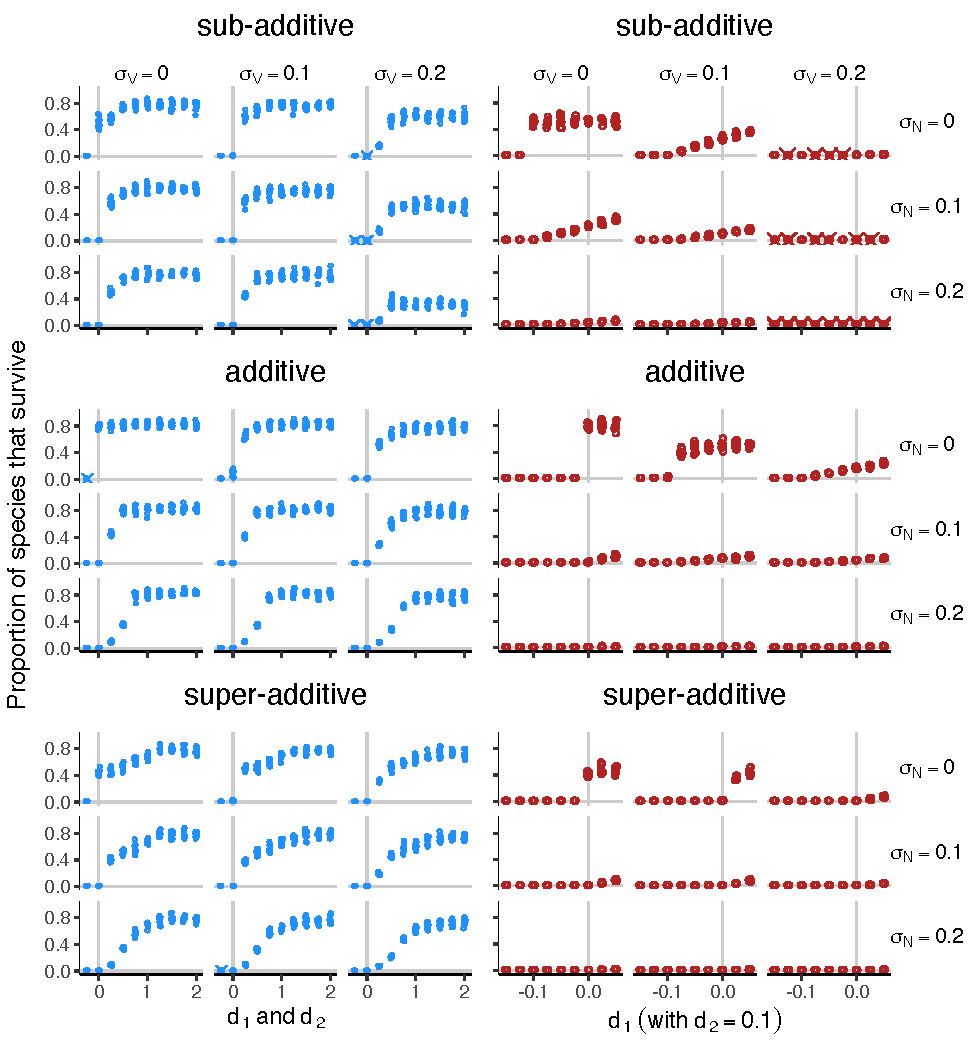
\includegraphics[width=0.9\textwidth]{S3-stoch_coexist.pdf}
\caption{Proportion of species that survived in simulations of 100-species, 2-axis
    communities with
    (A) varying $d_1$ and $d_2$ or 
    (B) varying just $d_1$ with $d_2$ fixed at 0.1.
    Standard deviations are for stochasticity in
    population dynamics ($\sigma_N$) and
    axis evolution ($\sigma_V$).
    Shown for sub-additive ($\eta < 0$), additive ($\eta = 0$), and 
    super-additive ($\eta > 0$) tradeoffs.
    Additive genetic variance ($\sigma_i^2$) was fixed at 0.05 for 
    these simulations.}
\label{fig:stoch-coexist-nspp}
\end{figure}



\begin{figure}[ht!]
\centering
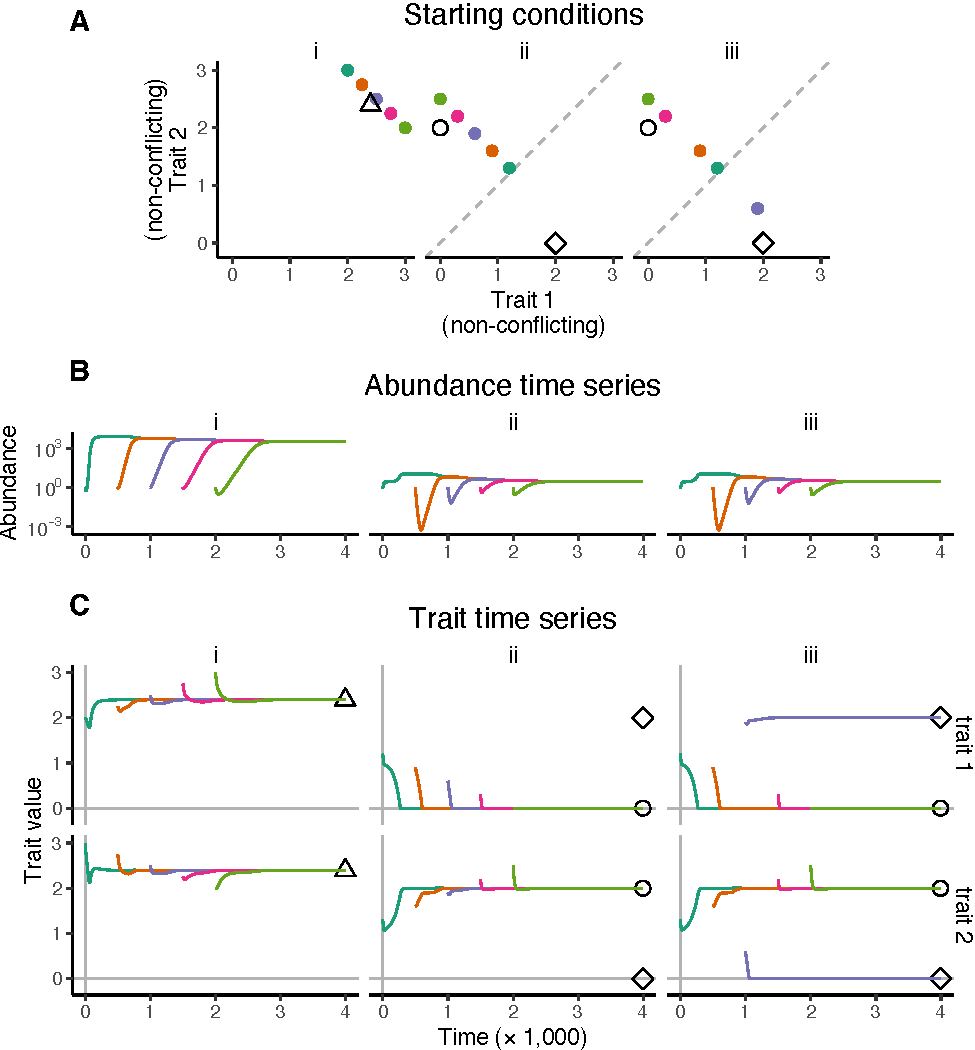
\includegraphics[width=0.7\textwidth]{S1-cond_coexist_non-conflicting.pdf}
\caption{Coexistence for 2-axis, 5-species communities when
    both axes have non-conflicting evolution.
    Panels show, for each of five situations,
    (A) starting conditions and trajectories for each species in axis space, 
    (B) abundances through time, and 
    (C) axis values through time.
    Situation i has sub-additive tradeoffs, situations ii and iv have 
    super-additive, and iii and v have additive.
    (A) Dashed arcs show the location of neutrally stable rings
    when tradeoffs are additive, and 
    the dotted lines separate the basins of attraction for the two possible
    axis states when tradeoffs are super-additive.
    (A,C) Shapes of hollow points indicate the equilibrium axis state.
    (C) For situations iii and v, line width is proportional to the 
    distance from the neutrally stable ring.}
\label{fig:cond-coexist-non-conflicting}
\end{figure}


\begin{figure}[ht!]
\centering
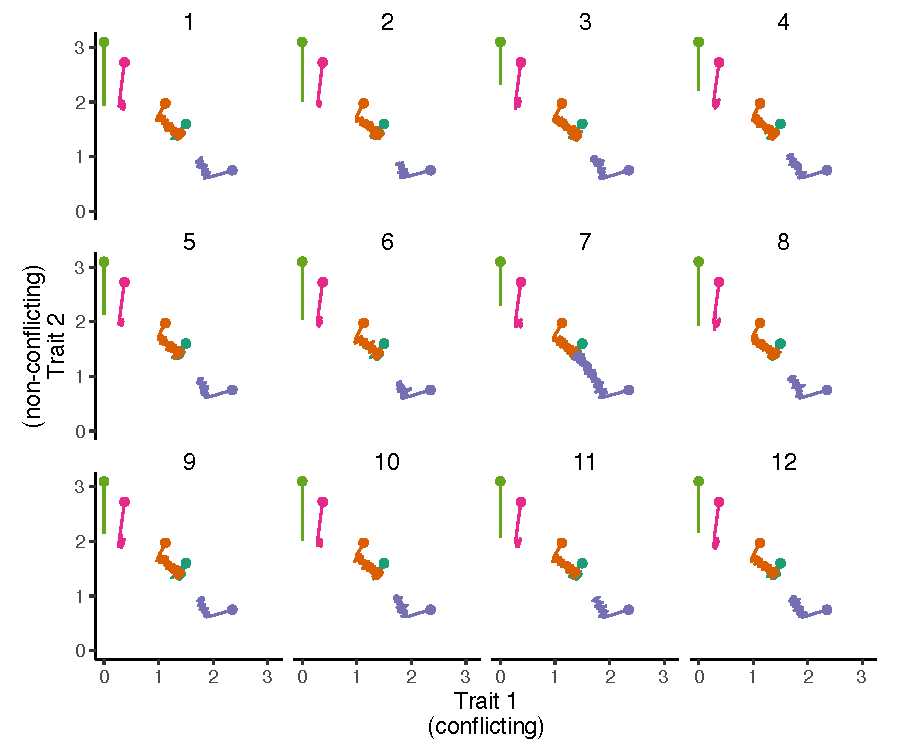
\includegraphics{S2-cc_sigmaV_sit_v.pdf}
\caption{Genotype trajectories through axis space for 12 repetitions under 
scenario v (see main text), with axis stochasticity ($\sigma_V = 0.1$).
Points indicate starting locations, and color indicates species.}
\label{fig:cond-coexist-Vstoch-sit-v}
\end{figure}



\begin{figure}[ht!]
\centering
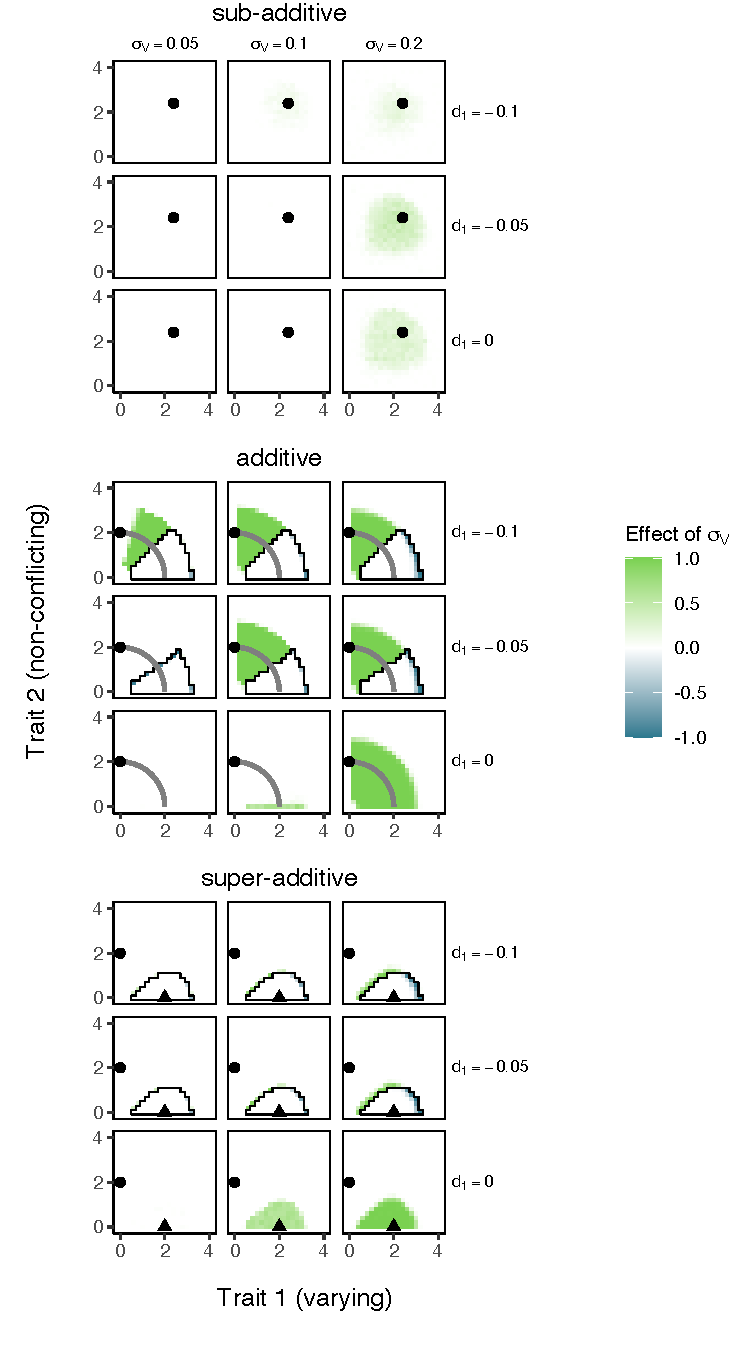
\includegraphics[width=0.5\textwidth]{S4-inv_sims_hm_replace.pdf}
\caption{Effect of stochasticity on replacement of resident species by invader
    based on the invader's starting axis values (x and y axes),
    magnitude of stochasticity (sub-panel columns), and 
    value of $d_1$ (sub-panel rows).
    Shown for sub-additive, additive, and super-additive tradeoffs.}
\label{fig:inv-sims-heatmap-replace}
\end{figure}

\begin{figure}[ht!]
\centering
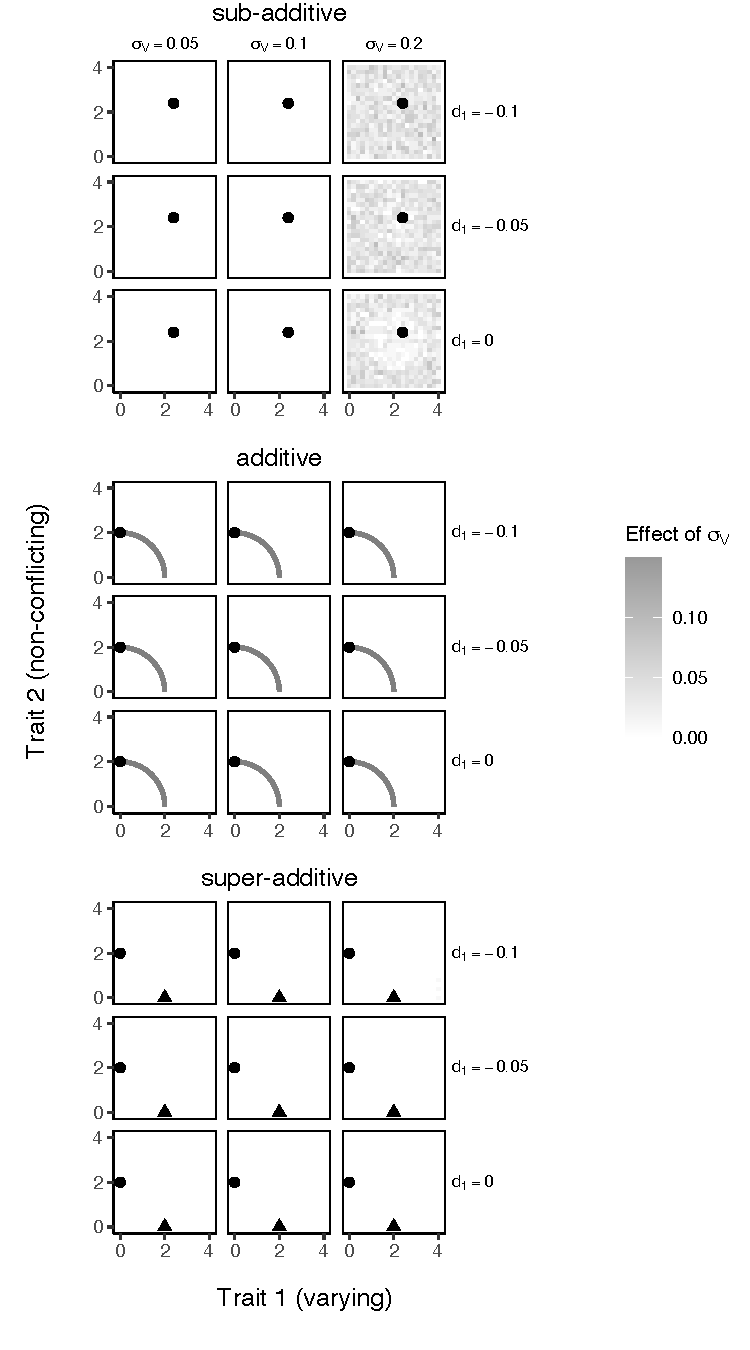
\includegraphics[width=0.5\textwidth]{S5-inv_sims_hm_extinct.pdf}
\caption{Effect of stochasticity on extinction of both resident and invader
    species based on the invader's starting axis values (x and y axes),
    magnitude of stochasticity (sub-panel columns), and 
    value of $d_1$ (sub-panel rows).
    Shown for sub-additive, additive, and super-additive tradeoffs.}
\label{fig:inv-sims-heatmap-extinct}
\end{figure}




\end{document}
